\section{Раздел 11: Именованные величины решения.}
1. Собака догоняет лису со скоростью $200-160=40$м/мин, значит ей понадобится $200:40=5$ минут.\\
2. Волк догоняет зайца со скоростью $200-160=40$м/мин, значит ему понадобится $200:40=5$ минут.\\
3. Найдём другую сторону:$b=P:2-a=30:2-10=5$см.\\
4. Найдём другую сторону:$b=P:2-a=30:2-5=10$см.\\
5. Раз кирпич весит как полкирпича и ещё 1 кг, половина кирпича весит как раз 1 кг. Значит, один кирпич весит 2кг, а 5 кирпичей весят $2\cdot5=10$кг.\\
6. Раз лещ весит как поллеща и ещё 2 кг, половина леща весит как раз 2 кг. Значит, один лещ весит 4кг, а 2 леща весят $4\cdot2=8$кг.\\
7. Пусть меньший кусок $x$м, тогда больший $4x$м. Значит, $x+4x=35,\ 5x=35,\ x=7$м.\\
8. Пусть меньший кусок $x$м, тогда больший $4x$м. Значит, $x+4x=45,\ 5x=45,\ x=9,\ 4x=36$м.\\
9. Раз периметр квадрата равен 16дм, его сторона равна $16:4=4$дм. Тогда у получившегося прямоугольника стороны равны 4дм и $4\cdot2=8$дм, а значит его периметр
равен $(4+8)\cdot2=24$дм.\\
10. Раз периметр квадрата равен 16дм, его сторона равна $16:4=4$дм. Тогда у получившегося прямоугольника стороны равны 4дм и $4\cdot2=8$дм, а значит его
площадь равна $4\cdot8=32\text{дм}^2.$\\
11. Раз скорость мотоцикла в 2 раза больше, времени он потратит в 2 раза меньше, то есть $4:2=2$ч.\\
12. Поезду осталось проехать $700-3\cdot70-2\cdot85=320$км за $9-3-2=4$ч. Значит, ему надо ехать со скоростью $320:4=80$км/ч.\\
13. Пятачок принёс в 3 раза меньше мёда, то есть $1080:3=360$г, то есть меньше Кролика на $1080-360=720$г. С другой стороны, он принёс меньше на 8 банок, а значит в одной банке содержится $720:8=90$г мёда. Поэтому Пятачок принёс $360:90=4$ банки, а Кролик $4+8=12$ банок. Таким образом, всего Пух получил $4+12=16$ банок.\\
14. Найдём другую сторону: $b=S:a=30:10=3$см. А значит, $P=(a+b)\cdot2=(10+3)\cdot2=26$см.\\
15. Найдём другую сторону: $b=S:a=24:3=8$см. А значит, $P=(a+b)\cdot2=(8+3)\cdot2=22$см.\\
16. Раз периметр квадрата равен 10м, его сторона равна $10\text{м}:4=100\text{дм}:4=25$дм. Тогда сторона большого квадрата равна $25\cdot2=50\text{дм}=5\text{м},$ а значит его периметр равен $5\cdot4=20$м.\\
17. Раз периметр квадрата равен 14м, его сторона равна $14\text{м}:4=140\text{дм}:4=35$дм. Тогда сторона большого квадрата равна $35\cdot2=70\text{дм}=7\text{м},$ а значит его периметр равен $7\cdot4=28$м.\\
18. Раз скорость мотоцикла в 3 раза больше, времени он потратит в 3 раза меньше, то есть $6:3=2$ч.\\
19. Раз скорость велогонщика в 4 раза меньше, времени он потратит в 4 раза больше, то есть $6\cdot4=24$ч.\\
20. Меньше всего кваса во второй бочке, значит в первой $14+3=17$л, а в третьей --- $17+5=22$л. Таким образом, всего в трёх бочках содержится $17+14+22=53$л кваса.\\
21. Меньше всего орехов в третьем ящике, значит в первом $13+9=22$кг, а во втором --- $22+4=26$кг. Таким образом, всего в трёх ящиках содержится $22+26+13=61$кг орехов.\\
22.$P_{\text{пр}}=(6+12)\cdot2=36$см. Значит, сторона квадрата $a=36:4=9$см.\\
23.$P_{\text{пр}}=(13+23)\cdot2=72$см. Значит, сторона квадрата $a=72:4=18$см.\\
24.$b=S:a=7500\text{дм}^2:15\text{м}=7500\text{дм}^2:150\text{дм}=50\text{дм}=5$м.\\
25.$b=S:a=2600\text{см}^2:13\text{дм}=2600\text{см}^2:130\text{см}=20\text{см}=2$дм.\\
26. За 1 час 30 минут Ваня пройдёт $4+2=6$км. Петя догоняет его со скоростью $6-4=2$км/ч, а значит ему понадобится $6:2=3$ч.\\
27. За 20 минут Таня пройдёт $6:3=2$км. Мама догоняет её со скоростью $8-6=2$км/ч, а значит ей понадобится $2:2=1$ч.\\
28. Найдём длину: $a=12+4=16$см. Тогда $P=(12+16)\cdot2=56$см, $S=12\cdot16=192\text{см}^2.$\\
29. Найдём ширину: $b=18-5=13$см. Тогда $P=(18+13)\cdot2=62$см, $S=18\cdot13=234\text{см}^2.$\\
30. Вместе бобры грызут ствол со скоростью $55+65=120$см/ч. Значит, за 2 часа 30 минут они сгрызут $120\cdot2+120:2=300\text{см}=3$м.\\
31. Шапокляк догоняла Гену со скоростью $105:3=35$км/ч, значит его скорость равна $90-35=55$км/ч.\\
32. Коля: $8:00+00:11=8:11$, Серёжа: $8:11-00:06=8:05,$ Саша: $8:05-00:09=7:56.$ Значит, порядок такой: Саша, Петя, Серёжа, Коля.\\
33. Коля: $7:00-00:13=6:47,$ Серёжа: $6:47+00:04=6:51,$ Саша: $6:51+00:10=7:01.$ Значит, порядок такой: Коля, Серёжа, Петя, Саша.\\
34. Сторона квадрата: $a_{\text{кв}}=40:4=10$см. Тогда площадь квадрата и прямоугольника $S=10\cdot10=100\text{см}^2.$ Значит, его вторая сторона $b=100:20=5$см.\\
35. Сторона квадрата: $a_{\text{кв}}=32:4=8$см. Тогда площадь квадрата и прямоугольника $S=8\cdot8=64\text{см}^2.$ Значит, его вторая сторона $b=64:4=16$см.\\
36. Пусть с момента вылета самолёта лайнер проплыл $x$км, тогда самолёт за это время пролетел $10x$км (так как его скорость в 10 раз больше). Самолёт догонит лайнер, если они окажутся на одинаковом расстоянии от берега, то есть $x+180=10x,\ 180=9x,\ x=20$км. Таким образом, самолёт догонит лайнер на расстоянии $180+20=200$км от берега.\\
37. Пусть с момента выезда мотоциклиста велосипедист проехал $x$км, тогда мотоциклист за это время проехал $3x$км (так как его скорость в 3 раза больше). Мотоциклист догонит велосипедиста, если они окажутся на одинаковом расстоянии от посёлка, то есть $x+300=3x,\ 300=2x,\ x=150$м. Таким образом, мотоциклист догонит велосипедиста на расстоянии $300+150=450$м от посёлка.\\
38. Найдём сторону квадрата: $a_{\text{кв}}=18\text{дм}:4=180\text{см}:4=45$см. Значит, стороны прямоугольника равны $45$ см и $45\cdot3=135$см. Поэтому его периметр $P=(45+135)\cdot2=360\text{см}=36$дм, а площадь --- $S=45\cdot135=6075\text{см}^2.$\\
39. Найдём сторону квадрата: $a_{\text{кв}}=14\text{дм}:4=140\text{см}:4=35$см. Значит, стороны прямоугольника равны $35$ см и $35\cdot3=105$см. Поэтому его периметр $P=(35+105)\cdot2=280\text{см}=28$дм, а площадь --- $S=35\cdot105=3675\text{см}^2.$\\
40. Раз скорость велосипедиста в 5 раз больше, времени он потратит в 5 раз меньше: $3\text{ч}:5=180\text{мин}:5=36$мин.\\
41. Раз скорость мотоциклиста в 12 раз больше, времени он потратит в 12 раз меньше: $7\text{ч}:12=420\text{мин}:12=35$мин.\\
42. Сначала оценим: 700 дней --- это два года без 30 дней $(700=365\cdot2-30),$ високосными годами в данном случае можно пренебречь, даже если бы они имелись. Если бы прошло ровно два года, то было бы 18 мая 2016 года. Так как прошло на 30 дней меньше, будет апрель 2016 года. Чтобы определить день недели, надо узнать, какой остаток число 700 даёт при делении на 7: $700:7=100.$Так как остатка нет, пройдёт ровно 100 недель и день недели опять будет воскресеньем.\\
43. Сначала оценим: 700 дней --- это два года без 30 дней $(700=365\cdot2-30),$ високосными годами в данном случае можно пренебречь, даже если бы они имелись. Если бы мы переместились в прошлое ровно на два года, то было бы 18 мая 2012 года. Так как прошло на 30 дней меньше, будет июнь 2012 года (двигаемся во времени назад, один месяц не добираемся до мая). Чтобы определить день недели, надо узнать, какой остаток число 700 даёт при делении на 7: $700:7=100.$Так как остатка нет, ровно 100 недель назад также было воскресенье.\\
44. Посчитаем, сколько времени поезд тратит на поездку из Москвы в Талдан и обратно. С $00-35$ до $18-15$ проходит 17 часов 40 минут, а с $8-23$ до $14-03$ проходит 5 часов 40 минут. На самом деле, конечно, в обоих случаях проходит ещё некоторое количество полных суток, для нас важно то, что это количество одинаковое в обоих случаях (поезд едет по одному маршруту с одинаковой скоростью). Поэтому разница в потраченном на эти поездки времени составляет $17:40-5:40=12$ часов. За счёт чего появилась эта разница, если поезд едет по тому же маршруту с той же скоростью? Всё дело в том, что Талдан находится восточнее Москвы, соответственно лежит в другом часовом поясе и когда поезд приезжает из Москвы в Талдан, разница во времени прибавляется к текущему времени, а на пути назад, наоборот, вычитается. Поэтому и получилось, что на поездку из Москвы в Талдан поезд тратит на 12 часов больше, чем на обратную дорогу. Если поезд проводит в дороге $t$ часов, а разница во времени составляет $x$ часов, то верно соотношение: $(t+x)-(t-x)=12,\ 2x=12, x=6$ч. Таким образом, разница во времени между Москвой и Талданом составляет 6 часов.\\
45. Посчитаем, сколько времени поезд тратит на поездку из Ярославля в Лучегорск и обратно. С $04-45$ до $19-05$ проходит 14 часов 20 минут, а с $8-25$ до $8-45$ проходит 20 минут. На самом деле, конечно, в обоих случаях проходит ещё некоторое количество полных суток, для нас важно то, что это количество одинаковое в обоих случаях (поезд едет по одному маршруту с одинаковой скоростью). Поэтому разница в потраченном на эти поездки времени составляет $14:20-0:20=14$ часов. За счёт чего появилась эта разница, если поезд едет по тому же маршруту с той же скоростью? Всё дело в том, что Лучегорск находится восточнее Ярославля, соответственно лежит в другом часовом поясе и когда поезд приезжает из Ярославля в Лучегорск, разница во времени прибавляется к текущему времени, а на пути назад, наоборот, вычитается. Поэтому и получилось, что на поездку из Ярославля в Лучегорск поезд тратит на 14 часов больше, чем на обратную дорогу. Если поезд проводит в дороге $t$ часов, а разница во времени составляет $x$ часов, то верно соотношение: $(t+x)-(t-x)=14,\ 2x=14, x=7$ч. Таким образом, разница во времени между Ярославлем и Лучегорском составляет 7 часов.\\
46. Найдём вторую сторону $b=14\text{м}+3\text{см}=1400\text{см}+3\text{см}=1403\text{см}.$ Тогда $P=(1400+1403)\cdot2=5606$см, $S=1400\cdot1403=1964200\text{см}^2.$\\
47. Найдём вторую сторону $b=13\text{м}+4\text{см}=1300\text{см}+4\text{см}=1304\text{см}.$ Тогда $P=(1300+1304)\cdot2=5208$см, $S=1300\cdot1304=1695200\text{см}^2.$\\
48. Если турист побежит назад в 5 раз быстрее, то он на обратную дорогу потратит в 5 раз меньше времени: $11\text{ч}:5=660\text{мин}:5=132\text{мин}=2-12.$ Таким образом, он вернётся в $9-15+11-00+2-12=22-27.$\\
49. Если турист побежит назад в 6 раз быстрее, то он на обратную дорогу потратит в 6 раз меньше времени: $8\text{ч}:6=480\text{мин}:6=80\text{мин}=1-20.$ Таким образом, он вернётся в $11-45+8-00+1-20=21-05.$\\
50. Сначала оценим: 1060 дней --- это три года без 35 дней $(1060=365\cdot3-35),$ високосными годами в данном случае можно пренебречь. Если бы прошло ровно три года, то было бы 17 мая 2018 года. Так как прошло на 35 дней меньше, будет апрель 2018 года. Чтобы определить день недели, надо узнать, какой остаток число 1060 даёт при делении на 7: $1060:7=151 (\text{ост. } 3).$Так как остаток равен 3, пройдёт ровно 151 неделя и ещё 3 дня, значит к воскресенью надо добавить 3 дня. Таким образом, искомый день будет средой.\\
51. Сначала оценим: 1060 дней --- это три года без 35 дней $(1060=365\cdot3-35),$ високосными годами в данном случае можно пренебречь. Если бы мы переместились в прошлое ровно на три года, то было бы 17 мая 2012 года. Так как прошло на 35 дней меньше, будет июнь 2012 года (двигаемся во времени назад, один месяц не добираемся до мая). Чтобы определить день недели, надо узнать, какой остаток число 1060 даёт при делении на 7: $1060:7=151 (\text{ост. } 3).$Так как остаток равен 3, мы перемещаемся назад на 151 неделю и ещё 3 дня, значит от воскресенья надо отнять 3 дня. Таким образом, искомый день будет четвергом.\\
52. Так как 2012 делится на 4, этот год является високосным, а значит в нём присутствует 29 февраля. Посчитаем, сколько Вася будет готовиться в каждый из дней: 26 февраля $2-05$; 27, 28 и 29 февраля по $24-00$; 1 марта $8-07.$ Таким образом, всего он потратит на подготовку $2-05+24-00+24-00+24-00+8-07=82\text{ часа }12\text{ минут.}$\\
53. Так как 2012 делится на 4, этот год является високосным, а значит в нём присутствует 29 февраля. Посчитаем, сколько Вася будет готовиться в каждый из дней: 27 февраля $4-25$; 28, 29 февраля и 1 марта по $24-00$; 2 марта $9-13.$ Таким образом, всего он потратит на подготовку $4-25+24-00+24-00+24-00+9-13=85\text{ часов }38\text{ минут.}$\\
54. Найдём вторую сторону: $b=11\text{м}+13\text{дм}=110\text{дм}+13\text{дм}=123$дм. Тогда $P=(110+123)\cdot2=466$дм.\\
55. Найдём вторую сторону: $b=13\text{м}+11\text{дм}=130\text{дм}+11\text{дм}=141$дм. Тогда $P=(130+141)\cdot2=542$дм.\\
56. Если в одном футе 12 дюймов, в одном квадратном футе $12\cdot12=144$ квадратных дюйма. Тогда в трёх квадратных футах $144\cdot3=432$ квадратных дюйма.\\
57. Если в одной сажени 7 футов, в одной квадратной сажени $7\cdot7=49$ квадратных футов. Тогда в 8 квадратных саженях $49\cdot8=392$ квадратных фута.\\
58. Стакан меньше банки в $3\text{л}:250\text{мл}=3000\text{мл}:250\text{мл}=12$ раз. Значит, на его заполнение уйдёт в 12 раз меньше времени: $7\text{мин}:12=420\text{сек}:12=35$ секунд.\\
59. Стакан меньше банки в $5\text{л}:250\text{мл}=5000\text{мл}:250\text{мл}=20$ раз. Значит, на его заполнение уйдёт в 20 раз меньше времени: $9\text{мин}:20=540\text{сек}:20=27$ секунд.\\
60. Оценим, сколько пройдёт дней: $280\text{ч}:24=11$(ост. 16). Так как начало отсчёта в полдень, 16 часов из остатка добавят ещё один день и пройдёт не 11, а 12 дней. Таким образом, будет $22\text{ мая }+12\text{ дней }=34\text{ мая }=3\text{ июня}.$ Так как 12 при делении на 7 даёт остаток 5, днём недели будет $\text{воскресенье }+5\text{ дней }=\text{ пятница.}$\\
61. Оценим, сколько пройдёт дней: $310\text{ч}:24=12$(ост. 22). Так как начало отсчёта в полдень, 22 часа из остатка добавят ещё один день и пройдёт не 12, а 13 дней. Таким образом, будет $22\text{ мая }+13\text{ дней }=35\text{ мая }=4\text{ июня}.$ Так как 13 при делении на 7 даёт остаток 6, днём недели будет $\text{воскресенье }+6\text{ дней }=\text{ суббота.}$\\
62. Так как 1944 делится на 4, этот год является високосным, а значит в нём присутствует 29 февраля. То есть февраль состоит из 4 полных недель (в них всех дней недели поровну) и ещё одного дня, 29 февраля: какой день недели выпадет на эту дату, тот и будет искомым. Раз 13 марта был понедельник, 15 марта было средой, как и 1 марта (ровно две недели назад). Тогда 29 февраля было вторником.\\
63. Так как 1944 делится на 4, этот год является високосным, а значит в нём присутствует 29 февраля. То есть февраль состоит из 4 полных недель (в них всех дней недели поровну) и ещё одного дня, 29 февраля: какой день недели выпадет на эту дату, тот и будет искомым. Раз 16 марта была суббота, 15 марта было пятницей, как и 1 марта (ровно две недели назад). Тогда 29 февраля было четвергом.\\
64. Формула для нахождения периметра $P=(a+b)\cdot2$ подразумевает, что значение периметра является чётным числом. Поэтому необходимо перевести все величины из метров в дециметры: $P=21\text{м}=210\text{дм},\ S=5\text{м}^2=500\text{дм}^2.$ Тогда необходимо придумать такие числа $a$ и $b,$ чтобы выполнялись равенства $(a+b)\cdot2=210,\ a\cdot b=500.$ Из первого равенства следует, что $a+b=105$ и нетрудно подобрать числа $a=100, b=5.$ Таким образом, ответом будет 100дм или 10м.\\
65. Формула для нахождения периметра $P=(a+b)\cdot2$ подразумевает, что значение периметра является чётным числом. Поэтому необходимо перевести все величины из метров в дециметры: $P=29\text{м}=290\text{дм},\ S=7\text{м}^2=700\text{дм}^2.$ Тогда необходимо придумать такие числа $a$ и $b,$ чтобы выполнялись равенства $(a+b)\cdot2=290,\ a\cdot b=700.$ Из первого равенства следует, что $a+b=145$ и нетрудно подобрать числа $a=140, b=5.$ Таким образом, ответом будет 140дм или 14м.\\
66. Когда у Васи $15-00,$ у Пети $9-00,$ то есть у Васи времени больше на 6 часов. Тогда если у Пети 3 часа ночи, у Васи 9 часов утра.\\
67. Когда у Васи $10-00,$ у Пети $15-00,$ то есть у Пети времени больше на 5 часов. Тогда если у Пети 9 часов утра, у Васи 4 часа ночи.\\
68. Найдём вторую сторону: $b=6\text{м}^2:12\text{м}=600\text{дм}^2:120\text{дм}=5\text{дм}.$ Тогда $P=(120+5)\cdot2=250\text{дм}=25\text{м}.$\\
69. Найдём вторую сторону: $b=8\text{м}^2:16\text{м}=800\text{дм}^2:160\text{дм}=5\text{дм}.$ Тогда $P=(160+5)\cdot2=330\text{дм}=33\text{м}.$\\
70. Пусть настоящее время $12-00.$ Тогда часы Леонида показывают $12-10,$ а он думает, что сейчас уже $12-15.$ Значит, чтобы прийти на встречу вовремя, он придёт на 15 минут раньше (так как к настоящему времени он прибавляет 15 минут). Часы Юлии в то же время показывают $11-55,$ а она думает, что сейчас уже $12-30.$ Поэтому она придёт раньше на 30 минут и будет ждать Леонида 15 минут.\\
71. Пусть настоящее время $12-00.$ Тогда часы Леонида показывают $12-10,$ а он думает, что сейчас уже $12-05.$ Значит, чтобы прийти на встречу вовремя, он придёт на 5 минут раньше (так как к настоящему времени он прибавляет 5 минут). Часы Юлии в то же время показывают $11-35,$ а она думает, что сейчас только $11-20.$ Поэтому она придёт позже на 40 минут и Леонид будет ждать её 45 минут.\\
72. В задаче не дано, каким был год: високосным или нет. Поэтому необходимо разобрать два случая. Рассмотрим следующую цепочку:
$10.01\stackrel{+31}{\rightarrow}10.02\stackrel{+28(29)}{\rightarrow}10.03.$ В невисокосном году до 10.03 пройдёт $31+28=59$ дней, а в високосном --- $31+29=60$ дней. Число 59 даёт при делении на 7 остаток 3, а число 60 --- остаток 4. Значит, в невисокосном году к понедельнику надо прибавить 3 дня, а в високосном --- 4. Поэтому в невисокосном году 10.03 будет четвергом, а в високосном --- пятницей. Тогда ближайшая суббота в невисокосном году будет 12.03, а в високосном --- 11.03. Последняя суббота марта наступит через 2 недели, то есть 26.03 в невисокосном году и 25.03 в високосном.\\
73. В задаче не дано, каким был год: високосным или нет. Поэтому необходимо разобрать два случая. Рассмотрим следующую цепочку:
$9.01\stackrel{+31}{\rightarrow}9.02\stackrel{+28(29)}{\rightarrow}9.03.$ В невисокосном году до 9.03 пройдёт $31+28=59$ дней, а в високосном --- $31+29=60$ дней. Число 59 даёт при делении на 7 остаток 3, а число 60 --- остаток 4. Значит, в невисокосном году ко вторнику надо прибавить 3 дня, а в високосном --- 4. Поэтому в невисокосном году 9.03 будет пятницей, а в високосном --- субботой. Тогда ближайшая пятница в невисокосном году так и будет 9.03, а в високосном --- 8.03. Последняя пятница марта наступит через 3 недели, то есть 30.03 в невисокосном году и 29.03 в високосном.\\
74. Раз обратно турист шёл в 2 раза быстрее, времени на дорогу он потратил в 2 раза меньше. Пусть обратно он шёл $x$ часов, тогда туда он шёл $2x$ часов, исходя из этого $x+2x=6,\ 3x=6,\ x=2$ч. Поэтому обратно его путь составил $4\cdot2=8$км, а значит весь путь был $2\cdot8=16$км.\\
75. Раз обратно турист шёл в 3 раза быстрее, времени на дорогу он потратил в 3 раза меньше. Пусть обратно он шёл $x$ часов, тогда туда он шёл $3x$ часов, исходя из этого $x+3x=8,\ 4x=8,\ x=2$ч. Поэтому обратно его путь составил $6\cdot2=12$км, а значит весь путь был $2\cdot12=24$км.\\
76. Раз аквариум заполнен наполовину, объём воды в нём равен $120:2=60\text{л}=60\text{дм}^3.$ Вода, разлитая по комнате, примет форму прямоугольного параллелепипеда, длина и ширина которого равны длине и ширине комнаты, а высота равна искомой высоте слоя воды. Так как объём прямоугольного параллелепипеда вычисляется по формуле $V=a\cdot b\cdot c,$ для нахождения его высоты необходимо поделить объём на произведение длины и ширины: $c=60\text{дм}^3:(3\text{м}\cdot4\text{м})=60\text{дм}^3:12\text{м}^2=60\text{дм}^3:1200\text{дм}^2=60000\text{см}^3:120000\text{см}^2=60000000\text{мм}^3:12000000\text{мм}^2=
5\text{мм}.$ Перевод в более мелкие единицы необходимо было осуществлять до тех пор, пока делимое не станет больше делителя. Для упрощения записи одинаковое количество нулей в делимом и делителе можно в процессе зачёркивать.\\
77. Раз аквариум заполнен наполовину, объём воды в нём равен $120:2=60\text{л}=60\text{дм}^3.$ Вода, разлитая по комнате, примет форму прямоугольного параллелепипеда, длина и ширина которого равны длине и ширине комнаты, а высота равна искомой высоте слоя воды. Так как объём прямоугольного параллелепипеда вычисляется по формуле $V=a\cdot b\cdot c,$ для нахождения его высоты необходимо поделить объём на произведение длины и ширины: $c=60\text{дм}^3:(3\text{м}\cdot5\text{м})=60\text{дм}^3:15\text{м}^2=60\text{дм}^3:1500\text{дм}^2=60000\text{см}^3:150000\text{см}^2=60000000\text{мм}^3:15000000\text{мм}^2=
4\text{мм}.$ Перевод в более мелкие единицы необходимо было осуществлять до тех пор, пока делимое не станет больше делителя. Для упрощения записи одинаковое количество нулей в делимом и делителе можно в процессе зачёркивать.\\
78. Разница во времени между Санкт-Петербургом и Новосибирском составляет $7-3=4$ часа. Значит, по петербургскому времени самолёт приземлится в Новосибирске в $4:20-4:00=0:20.$ Поэтому полёт длился $0:20-20:05=4:15.$ На обратный путь самолёт тратит на 20 минут больше, то есть $4:15+0:20=4:35.$ Тогда с учётом разницы во времени в Санкт-Петербурге будет $20:55+4:35-4:00=21:30.$\\
79. Разница во времени между Петропавловком-Камчатским и Токио составляет $9-6=3$ часа. Значит, по токийскому времени самолёт приземлится в Петропавловске-Камчатском в $22:10-3:00=19:10.$ Поэтому полёт длился $19:10-17:20=1:50.$ На обратный путь самолёт тратит столько же времени. Тогда с учётом разницы во времени в Токио будет $8:30+1:50-3:00=7:20.$\\
80. Посчитаем площадь: $21\cdot30=630\text{см}^2$ весят 1800 граммов. Тогда $630:9=70\text{см}^2$ весят $1800:9=200$г. Искомый лист весит больше в $7\text{м}^2:70\text{см}^2=70000\text{см}^2:70\text{см}^2=1000$ раз, а значит весит $200\text{г}\cdot1000=200000\text{г}=200$кг.\\
81. Посчитаем площадь: $21\cdot30=630\text{см}^2$ весят 210 граммов. Тогда $630:21=30\text{см}^2$ весят $210:21=10$г. Искомый лист весит больше в $3\text{м}^2:30\text{см}^2=30000\text{см}^2:30\text{см}^2=1000$ раз, а значит весит $10\text{г}\cdot1000=10000\text{г}=10$кг.\\
82. В любом году март состоит из 31 дня, то есть 4 полных недель и ещё 3 дня. В полных неделях всех дней всегда поровну, значит в последних 3 днях есть воскресенье, но нет понедельника. Это возможно только если 31 марта было воскресеньем. Тогда 1 апреля было понедельником. Рассмотрим следующую цепочку:
$1.04\stackrel{+30}{\rightarrow}1.05\stackrel{+31}{\rightarrow}1.06\stackrel{+12}{\rightarrow}13.06.$ С 1 апреля до 13 июня пройдёт $30+31+12=73$ дня. Число 73 даёт при делении на 7 остаток 3, значит к понедельнику надо прибавить 3 дня, а значит $13.06$ будет четвергом.\\
83. В любом году май состоит из 31 дня, то есть 4 полных недель и ещё 3 дня. В полных неделях всех дней всегда поровну, значит в последних 3 днях есть воскресенье, но нет понедельника. Это возможно только если 31 мая было воскресеньем. Тогда 1 июня было понедельником. Рассмотрим следующую цепочку:
$1.06\stackrel{+30}{\rightarrow}1.07\stackrel{+31}{\rightarrow}1.08\stackrel{+11}{\rightarrow}12.08.$ С 1 июня до 12 августа пройдёт $30+31+11=72$ дня. Число 72 даёт при делении на 7 остаток 2, значит к понедельнику надо прибавить 2 дня, а значит $12.08$ будет средой.\\
84. Посчитаем, сколько сначала времени между показаниями часов на башнях: $6-00+24-00+24-00+24-00+24-00+10-00=112-00$ (с $8.06$ по $13.06$ соответственно). Каждый час показания часов сближаются на 2 часа (отстающие часы идут на 1 час вперёд, а опережающие --- на 1 час назад, им навстречу). Таким образов, часы будут показывать одинаковое время через $112:2=56$ часов.\\
85. Посчитаем, сколько сначала времени между показаниями часов на башнях: $10-00+24-00+24-00+24-00+8-00=90-00$ (с $6.03$ по $10.03$ соответственно). Каждый час показания часов сближаются на 2 часа (отстающие часы идут на 1 час вперёд, а опережающие --- на 1 час назад, им навстречу). Таким образов, часы будут показывать одинаковое время через $90:2=45$ часов.\\
86. Площадь поверхности кубика равна $2\cdot2\cdot6=24\text{см}^2.$ А площадь поверхности ящика (он имеет форму прямоугольного параллелепипеда) равна $(4\cdot4+4\cdot7+4\cdot7)\cdot2=144\text{дм}^2=14400\text{см}^2,$ то есть она больше в $14400\text{см}^2:24\text{см}^2=600$ раз. Поэтому и краски понадобится больше в 600 раз: $370\text{мг}\cdot600=222000\text{мг}=222$г.\\
87. Площадь поверхности кубика равна $3\cdot3\cdot6=54\text{см}^2.$ А площадь поверхности ящика (он имеет форму прямоугольного параллелепипеда) равна $(3\cdot6+3\cdot7+6\cdot7)\cdot2=162\text{дм}^2=16200\text{см}^2,$ то есть она больше в $16200\text{см}^2:54\text{см}^2=300$ раз. Поэтому и краски понадобится больше в 300 раз: $730\text{мг}\cdot300=219000\text{мг}=219$г.\\
88. Второй человек вышел на 3 часа позже, первый за это время успел уйти на $4\cdot3=12$км. Всадник вёз письмо 45 минут, второй за это время пройдёт $3\cdot1=3$км (второй идёт со скоростью 4км/ч, то есть 1км/15мин). Значит, всадник проехал оставшиеся $12-3=9$км за 45 минут, то есть он проезжает 3км за 15мин или 12км за 1ч. Расстояние между первым и вторым человеком за это время не поменялось, так как они идут с одинаковой скоростью. За те полчаса, что он ждал ответа, первый человек увеличит расстояние между ними на $4:2=2$км и оно будет составлять $12+2=14$км. Всадник будет догонять первого человека со скоростью $12\text{км/ч}-4\text{км/ч}=8\text{км/ч}$ или 2км/15 мин. Поэтому на доставку ответа ему понадобится $14\text{км}:2\text{км/15мин}=7\cdot15\text{мин}=105\text{мин}=$1ч 45 мин.\\
89. Второй человек вышел на 2 часа позже, первый за это время успел уйти на $6\cdot2=12$км. Всадник вёз письмо 30 минут, второй за это время пройдёт $6:2=3$км. Значит, всадник проехал оставшиеся $12-3=9$км за 30 минут, то есть он проезжает $9\cdot2=18$км/ч. Расстояние между первым и вторым человеком за это время не поменялось, так как они идут с одинаковой скоростью. За те 40 минут, что он ждал ответа, первый человек увеличит расстояние между ними на $2\cdot2=4$км (первый идёт со скоростью 6км/ч, то есть 2км/20мин) и оно будет составлять $12+4=16$км. Всадник будет догонять первого человека со скоростью $18\text{км/ч}-6\text{км/ч}=12\text{км/ч}$ или 2км/10 мин. Поэтому на доставку ответа ему понадобится $16\text{км}:2\text{км/10мин}=8\cdot10\text{мин}=80\text{мин}=$1ч 20 мин.\\
90. Пусть ширина прямоугольника равна $x,$ тогда его длина равна $x+42$ и верно соотношение $(x+x+42)\cdot2=320,$ откуда $x=59\text{см}, x+42=101\text{см}.$ Таким образом, находим
$S=59\cdot101=5959\text{см}^2.$\\
91. Пусть ширина прямоугольника равна $x,$ тогда его длина равна $x+22$ и верно соотношение $(x+x+22)\cdot2=360,$ откуда $x=79\text{см},\ x+22=101\text{см}.$ Таким образом, находим
$S=79\cdot101=7979\text{см}^2.$\\
92. Раз между дном и крышкой помещается 3 кубика, высота коробки равна $3\cdot3=9$см. Так как высота составляет четверть ширины, а дно коробки квадратное, её длина и ширина равны $9\cdot4=36$см. Тогда её объём равен $9\cdot36\cdot36=11664\text{см}^3.$\\
93. Раз между дном и крышкой помещается 4 кубика, высота коробки равна $4\cdot2=8$см. Так как высота составляет треть ширины, а дно коробки квадратное, её длина и ширина равны $8\cdot3=24$см. Тогда её объём равен $8\cdot24\cdot24=4608\text{см}^3.$\\
94. За 8 дней 4 курицы снесут $4\cdot2=8$ яиц, а 8 куриц за 8 дней тогда снесут $8\cdot2=16$ яиц.\\
95. Если площадь квадрата равна $64\text{см}^2,$ его сторона равна $8\text{см}$ (так как $8\cdot8=64$). Значит, ширина прямоугольника равна $8:2=4\text{см}.$ Периметр квадрата равен $4\cdot8=32\text{см},$ значит периметр прямоугольника равен $4\cdot32=128$см. Тогда его длина равна $128:2-4=60$см. В таком случае восьмая
часть его площади равна $4\cdot60:8=30\text{см}^2.$\\
96. Пусть ширина участка равна $x,$ тогда его длина равна $x+12$ и верно равенство $(x+x+12)\cdot2=152,$ откуда $x=(152:2-12):2=32\text{м}.$ Тогда длинная сторона участка равна $32+12=44\text{м},$ а значит расстояние от середины ворот до угла участка равно $44:2=22\text{м}.$ Так как ширина ворот равна 2м, расстояние от края ворот до угла участка равно $22-2:2=21\text{м}.$\\
97. Пусть ширина участка равна $x,$ тогда его длина равна $x+15$ и верно равенство $(x+x+15)\cdot2=174,$ откуда $x=(174:2-15):2=36\text{м}.$ Значит расстояние от середины ворот до угла участка равно $36:2=18\text{м}.$ Так как ширина ворот равна 2м, расстояние от края ворот до угла участка равно $18-2:2=17\text{м}.$\\
98. Незнайка вскопал треть огорода, то есть $15\cdot49:3=245\text{м}^2.$ Тогда грядок было $245:7\cdot2=70$ штук.\\
99. Буратино вскопал четверть Поля Чудес, то есть $63\cdot20:4=315\text{м}^2.$ Тогда монет было посажено $315:9\cdot2=70$ штук.\\
100. Автобус догоняет самосвал со скоростью $100-80=20$км/ч. Тогда первая их встреча произойдёт через $60:20=3$ч. За это время автобус проедет $3\cdot100=300$км, а значит расстояние от санатория до порта равно $300+300=600$км. Автобус доедет до порта ещё через $300:100=3$ч, за это время самосвал проедет $80\cdot3=240$км. Тогда к тому моменту, как автобус в порту развернётся и поедет назад, расстояние между ними будет равно $300-240=60$км. Скорость их сближения будет равна $100+80=180$км/ч. Расстояние между ними равно трети от скорости их сближения, а значит до встречи пройдёт треть часа, то есть 20 минут. Таким образом, расстояние между санаторием и портом равно 600 км, а до второй встречи пройдёт $3\text{ч}+3\text{ч}+20\text{мин}=6\text{ч}20\text{мин}.$\\
101. Легковой автомобиль догоняет грузовик со скоростью $90-60=30$км/ч. Тогда первая их встреча произойдёт через $120:30=4$ч. За это время легковой автомобиль проедет $4\cdot90=360$км, а значит расстояние от города до деревни равно $360+90=450$км. Легковой автомобиль доедет до деревни ещё через $90:90=1$ч, за это время грузовик проедет $60\cdot1=60$км. Тогда к тому моменту, как легковой автомобиль в деревне развернётся и поедет назад, расстояние между ними будет равно $90-60=30$км. Скорость их сближения будет равна $90+60=150$км/ч. Расстояние между ними равно одной пятой от скорости их сближения, а значит до встречи пройдёт одна пятая часть часа, то есть 12 минут. Таким образом, расстояние между городом и деревней равно 450 км, а до второй встречи пройдёт $4\text{ч}+1\text{ч}+12\text{мин}=5\text{ч}12\text{мин}.$\\
102. Если Юля младше Оли, то старше её две девочки: Оля и Маша. Старше Оли она не может быть по условию, поэтому они родились в один день. Тогда самой старшей девочкой является Маша, а самой младшей --- Катя, причём Маша старше кати на $7+9=16$ дней.\\
103. Каждый раз длина полоски уменьшалась в 2 раза, для получения длины, равной 1см, полоску на сложить 6 раз (если 64 поделить на 2 шесть раз, получится 1).\\
104. В Киликуку времени больше на $12-9=3$ часа. Тогда в момент прибытия самолёта из Билибуку там будет $13:30+5:00+3:00=21:30.$\\
105. Периметр цветника составляет $50\cdot4=200$м. Ширина составляет 2/8 длины, то есть длина больше в 4 раза. Пусть ширина равна $x,$ тогда длина равна $4x$ и верно равенство $(x+4x)\cdot2=200,\ 5x=100,\ x=20$м. Тогда длина равна $4\cdot20=80$м, а площадь цветника $S=20\cdot80=1600\text{м}^2.$ Розами засадили 3/8 цветника, то есть $1600:8\cdot3=600\text{м}^2.$ Гладиолусами засадили 3/5 остатка, то есть $(1600-600):5\cdot3=600\text{м}^2.$ Значит, под незабудки осталось $1000-600=400\text{м}^2.$\\
106. Если площадь квадрата равна $x,$ то площадь прямоугольника с одной стороны равна $4x,$ а с другой стороны --- $x+432,$ откуда $4x=x+432,\ 3x=432,\ x=144\text{см}^2.$ Тогда сторона квадрата равна 12см (так как $12\cdot12=144$). Значит, ширина прямоугольника равна $12:4=3$см. Его площадь равна $144+432=576\text{см}^2,$ поэтому длина равна $576:3=192$ см. Тогда периметры квадрата и прямоугольника равны $P_\text{кв}=4\cdot12=48\text{см},\ P_\text{пр}=(3+192)\cdot2=390\text{см}.$ Таким образом, периметр прямоугольника больше на $390-48=342$см.\\
107. Если 17.06 было понедельником, то 17.07 было средой, так как прошло 30 дней, а число 30 даёт остаток 2 при делении на 7. Тогда ближайшая суббота была 20.07, а вторая в июле --- 13.07 (до неё была суббота только 6.07).\\
108. Если 13.05 было пятницей, то 13.06 было понедельником, так как прошёл 31 день, а число 31 даёт остаток 3 при делении на 7. Тогда третий понедельник в июне был 20.06 (до него были только понедельники 13.06 и 6.06).\\
109. Валера потратил 10г краски на $10\cdot10\cdot6=600\text{см}^2.$ Вася распилил большой куб на $10\cdot10\cdot10=1000$ маленьких кубиков, общая площадь поверхности которых равна $1\cdot1\cdot6\cdot1000=6000\text{см}^2,$ из которых $600\text{см}^2$ уже покрашены, а значит окрасить надо ещё $6000-600=5400\text{см}^2.$ Эта площадь больше в $5400:600=9$ раз, а значит краски потребуется больше в 9 раз: $10\cdot9=90$г.\\
110. Оля потратила 12г краски на $12\cdot12\cdot6=864\text{см}^2.$ Вася распилил большой куб на $12\cdot12\cdot12=1728$ маленьких кубиков, общая площадь поверхности которых равна $1\cdot1\cdot6\cdot1728=10368\text{см}^2,$ из которых $864\text{см}^2$ уже покрашены, а значит окрасить надо ещё $10368-864=9504\text{см}^2.$ Эта площадь больше в $9504:864=11$ раз, а значит краски потребуется больше в 11 раз: $11\cdot12=132$г.\\
111. Пересчитаем скорость: $120\text{м}/10\text{с}=720\text{м}/\text{мин}=43200\text{м}/\text{ч},$ а значит скорость была превышена.\\
112. Пересчитаем скорость: $130\text{м}/10\text{с}=780\text{м}/\text{мин}=46800\text{м}/\text{ч},$ а значит скорость не была превышена.\\
113. Так как каждый год Таня и Андрей суммарно становятся старше на 2 года, 15 лет им было $(21-15):2=3$ года назад. Раз Андрею 3 года назад было столько же лет, сколько Тане сейчас, он старше её на 3 года. Значит, тогда ему было $(15-3):2+3=9$ лет.\\
114. Так как каждый год Даша и Ксюша суммарно становятся старше на 2 года, 10 лет им было $(18-10):2=4$ года назад. Раз Даше 4 года назад было столько же лет, сколько Ксюше сейчас, она старше её на 4 года. Значит, тогда Ксюше было $(10-4):2=3$ года.\\
115. Пусть внучке Тане $x$ лет, тогда бабушке Оле $9x$ лет. Раз мама Аня находится посередине между внучкой и бабушкой, ей $5x$ лет. Тогда верно равенство $x+5x+9x=90,\ 15x=90,\ x=6$ лет. Поэтому бабушке Оле $9\cdot6=54$ года.\\
116. Снимем с обеих сторон весов по 3 рыжих кота. Тогда один рыжий кот с килограммовым пакетом весит столько же, сколько два двухкилограммовых пакета, откуда один кот весит 3 килограмма.\\
117. Снимем с обеих сторон весов по 2 белых котёнка. Тогда один белый котёнок и двухкилограммовый пакет весят столько же, сколько же, сколько три килограммовых пакета, откуда один котёнок весит 1 килограмм.\\
118. Если площадь салфетки больше в 4 раза, её сторона больше в 2 раза, а значит и периметр также больше в 2 раза. Значит, Вере потребуется $1\cdot2=2$ часа.\\
119. Рассмотри следующую цепочку: $1.04\stackrel{+30}{\rightarrow}1.05\stackrel{+31}{\rightarrow}1.06\stackrel{+30}{\rightarrow}1.07\stackrel{+31}{\rightarrow}1.08\stackrel{+31}{\rightarrow}1.09.$
С 1 апреля до 1 сентября пройдёт $30+31+30+31+31=153$ дня. Число 153 даёт остаток 6 при делении на 7, а значит ко вторнику надо прибавить 6 дней. Поэтому 1 сентября придётся на понедельник.\\
120. Дача Ивана имеет площадь (в $\text{дм}^2$) $649\cdot241=649\cdot(240+1)=649\cdot240+649.$ Посчитаем также в $\text{дм}^2$ площадь дачи Петра:
$650\cdot240=(649+1)\cdot240=649\cdot240+240.$ Таким образом, площадь дачи Ивана больше на $649-240=409\text{см}^2.$\\
121. Всего до веломагазина пешеход шёл $2:30+1:30=4$ часа. Так как его скорость на велосипеде в 3 раза больше, на обратный путь он потратит в 3 раза меньше времени: $4\text{ч}:3=240\text{мин}:3=80\text{мин}=1:20.$ Тогда домой он приедет в $10:00+2:30+1:00+1:30+0:30+1:20=16:50.$\\
122. Роботов станет больше в $10:2=5$ раз, а времени у них будет больше в $12:3=4$ раза. Значит, они соберут $1\cdot5\cdot4=20$ компьютеров.\\
123. Пересчитаем скорость: $200\text{м}/10\text{с}=1200\text{м}/\text{мин}=72000\text{м}/\text{ч}=72\text{км}/\text{ч}.$\\
124. Площадь поверхности кубика высотой 1 см равна $1\cdot1\cdot6=6\text{см}^2,$ а площадь поверхности кубика высотой 2 см равна $2\cdot2\cdot6=24\text{см}^2.$ Она больше в $24:6=4$ раза, а значит на второй кубик уйдёт $4\cdot1=4$г краски.\\
125. Пусть грузоподъёмность второго самосвала равна $x,$ тогда верно равенство $4x=x+24,\ 3x=24,\ x=8$т, а $x+24=32$т.\\
126. Пусть стороны прямоугольника равны $a$ и $b,$ тогда $(a+b)\cdot2=10,\ a+b=5$см. Тогда возможны два случая: стороны равны 2см и 3 см или 1см и 4см. Поэтому площадь может быть равна $2\cdot3=6\text{см}^2$ или $1\cdot4=4\text{см}^2.$\\
127. Если 700г яблок стоят 42 рубля, 100г яблок стоят $42:7=6$ рублей, а значит $1\text{кг}=1000$г яблок стоят $6\cdot10=60$ рублей.\\
128. Раз 20 машин делают по 12 рейсов, общее количество рейсов равно $20\cdot12=240.$ Тогда 15 машин должны будут сделать по $240:15=16$ рейсов.\\
129. Первая черепаха проползёт 20 метров за $9\cdot5=45$ минут, а вторая --- за $4\cdot11=44$ минуты. Значит, вторая черепаха ползёт быстрее.\\
130. Площадь квадрата равна $5\cdot5=25\text{см}^2.$ Тогда вторая сторона прямоугольника равна $25\text{см}^2:1\text{мм}=2500\text{мм}:1\text{мм}=2500\text{мм}=250\text{см}.$\\
131. Пересчитаем скорость: $15\text{м}/\text{с}=900\text{м}/\text{мин}.$ Тогда ему понадобится $27\text{км}:900\text{м}/\text{мин}=
27000\text{м}:900\text{м}/\text{мин}=30$мин.\\
132. Чтобы поезда разошлись, их начала с момента встречи должны разъехаться на расстояние, равное сумме их длин. Они будут удалять друг от друга со скоростью $6+5=11$м/с. Значит, им понадобится $(350+420):11=70$с.\\
133. Площадь квадрата (и прямоугольника) равна $2\cdot2=4\text{см}^2.$ Тогда вторая сторона прямоугольника равна $4\text{см}^2:2\text{мм}=400\text{мм}^2:2\text{мм}=
200\text{мм}=20$см.\\
134. Один учитель проверит эти работы за $4\cdot10=40$ часов, тогда 8 учителей справятся за $40:8=5$ часов.\\
135. Разница $5,5-2,5=3$ кг составляет 3/4 бидона, а значит всё молоко в бидоне весит $3:3\cdot4=4$ кг, поэтому сам бидон весит $5,5-4=1,5$кг.\\
136. Площадь поверхности кубика со стороной 1 см равна $1\cdot1\cdot6=6\text{см}^2,$ а площадь поверхности кубика со стороной 4 см равна $4\cdot4\cdot6=96\text{см}^2.$ Она больше в $96:6=16$ раз, а значит на второй кубик уйдёт $16\cdot7=112$г краски.\\
137. Пусть скорость автобуса равна $x,$ тогда скорость маршрутки равна $x+20$ и $(x+x+20)\cdot2=240,\ 2x+20=120,\ 2x=100,\ x=50$км/ч. Тогда скорость маршрутки равна $50+20=70$км/ч.\\
138. Если периметр равностороннего треугольника равен 21дм, его сторона равна $21:3=7\text{дм}.$ Тогда вторая сторона прямоугольника равна $3500\text{см}^2:7\text{дм}=35\text{дм}^2:7\text{дм}=5\text{дм}$. Сторона квадрата с площадью $64\text{дм}^2$ равна 8дм (так как $8\cdot8=64.$). Тогда его периметр (как и периметр прямоугольника) равен $8\cdot4=32$ дм. Возможны два случая: новый прямоугольник построен на стороне, равной 7дм, или на стороне, равной 5дм. В первом случае вторая сторона построенного прямоугольника равна $32:2-7=9$дм, а значит его площадь равна $7\cdot9=63\text{дм}^2.$ Во втором случае его вторая сторона равна $32:2-5=11$дм, а значит его площадь равна $5\cdot11=55\text{дм}^2.$\\
139. Если периметр равностороннего треугольника равен 9дм, его сторона равна $9:3=3\text{дм}.$ Тогда вторая сторона прямоугольника равна $2400\text{см}^2:3\text{дм}=24\text{дм}^2:3\text{дм}=8\text{дм}$. Сторона квадрата с площадью $36\text{дм}^2$ равна 6дм (так как $6\cdot6=36.$). Тогда его периметр (как и периметр прямоугольника) равен $6\cdot4=24$ дм. Возможны два случая: новый прямоугольник построен на стороне, равной 3дм, или на стороне, равной 8дм. В первом случае вторая сторона построенного прямоугольника равна $24:2-3=9$дм, а значит его площадь равна $3\cdot9=27\text{дм}^2.$ Во втором случае его вторая сторона равна $24:2-8=4$дм, а значит его площадь равна $8\cdot4=32\text{дм}^2.$\\
140. Раз расстояние между колобками через 30 секунд после столкновения стало равно 26 метров, скорость их удаления (равная сумме их скоростей) равна 52м/мин. Если скорость более медленного колобка равна $x,$ то скорость более быстрого --- $x+4$ и $x+x+4=52,\ 2x=48,\ x=24$м/мин. Значит, более быстрый колобок катится со скоростью $24+4=28$м/мин. Он удалялся от своей избушки 4 минуты и приближался к ней 30 секунд, то есть можно считать, что он удалялся 3 минуты и 30 секунд. Тогда он окажется на расстоянии $3\cdot28+28:2=98$м.\\
141. Раз расстояние между зайчатами через 30 секунд после столкновения стало равно 21 метру, скорость их удаления (равная сумме их скоростей) равна 42м/мин. Если скорость более медленного зайчонка равна $x,$ то скорость более быстрого --- $x+6$ и $x+x+6=42,\ 2x=36,\ x=18$м/мин. Значит, более быстрый зайчонок бежит со скоростью $18+6=24$м/мин. Он удалялся от своей норки 3 минуты и приближался к ней 30 секунд, то есть можно считать, что он удалялся 2 минуты и 30 секунд. Тогда он окажется на расстоянии $2\cdot24+24:2=60$м.\\
142. Пусть за первый промежуток времени Баба Яга пролетела $x$км, тогда за второй она пролетела $x+10$км, а за третий --- $x+10+20=x+30$км, и верно равенство $x+x+10+x+30=70,\ 3x=30,\ x=10$км. Так как все промежутки времени были равными, они составляли $45:3=15$мин. Таким образом, на втором промежутке Баба Яга пролетела $10+10=20$км за 15 минут, поэтому её скорость равна $20\cdot4=80$км/ч.\\
143. Вторая машина всего проехала 296км, значит в сторону пункта $C$ она проехала $296:2=148$км за 2 часа. Всего она должна была ехать 6 часов, значит до пункта $C$ ей оставалось ехать ещё 4 часа, за которые она проехала бы $148\cdot2=296$км. Поэтому первой машине через 2 часа после начала движения оставалось ехать до пункта $C$ ещё $628-296=332$км, которые она должна была бы проехать за 4 часа. Значит, за первые 2 часа она проехала $332:2=166$км. Таким образом, расстояние между пунктами $A$ и $C$ равно $166+332=498$км.\\
144. Раз площадь квадратной дощечки равна $64\text{см}^2,$ её сторона равна 8см (так как $8\cdot8=64$). Площадь полученного приложением прямоугольника равна $96\text{см}^2,$ а одна из его сторон равна стороне квадрата, то есть 8см. Поэтому вторая его сторона (полученная как сумма сторон квадрата и прямоугольника) равна $96\text{см}^2:8\text{см}=12$см, а значит это и есть большая сторона, которая равна одной из сторон треугольной дощечки. Периметр полученного прямоугольника равен $P=(12+8)\cdot2=40$см. У треугольной дощечки равны какие-то две стороны, а значит возможны два случая: две стороны по 12 см, а значит третья сторона равна $40-12\cdot2=16$см или две стороны по $x$ см, тогда $2x+12=40,\ 2x=28,\ x=14$см.\\
145. Расстояние от родника до каравана на 120м меньше, чем от родника о баобаба, значит от баобаба до каравана 120м. От путника до баобаба на 410м меньше, чем от путника до родника, значит от баобаба до родника 410м. Тогда от каравана до родника $410-120=290$м.\\
146. Пусть на приготовление пирога необходимо $x$ минут, тогда на приготовление пиццы их понадобится $x+4$ и $3x+x+4=60.\ 4x=56,\ x=14$мин. Значит, на пирог уходит 14мин, а на пиццу $14+4=18$мин. Если после пиццы делать перерыв 2 минуты, то на одну пиццу их будет уходить $18+2=20.$ Тогда за 2 с половиной часа можно сделать $(2\cdot60+60:2):20=150:20=7 (\text{ост. 10})$ пицц. За оставшиеся 10 минут ещё одну пиццу уже не сделать.\\
147. 21 ц 42 кг$\cdot3-8$ т 53 кг$:4=63\text{ ц }126\text{ кг }-2\text{ т }13\text{ кг }250\text{ г }=43\text{ ц }112\text{ кг }750\text{ г }=4412\text{ кг }750\text{ г}.$\\
148. 104 м 5 дм 3 см $\cdot 5-1$ км 16 м 35 см$:2=520\text{ м }25\text{ дм }15\text{ см }-508\text{ м }17\text{ см }5\text{ мм }=1447\text{ см }5\text{ мм}.$\\
149. Вова должен был проехать эти 144км за оставшиеся $5-2=3$ часа, значит его скорость $144:3=48$км/ч. Скорость их сближения равна $600:5=120$км/ч, значит скорость Алёши равна $120-48=72$км/ч. Алёше нужно проехать всё расстояние кроме того, которое успел проехать Вова за 2 часа, то есть $600-2\cdot48=504$км. Он проедет их за $504:72=7$ часов.\\
150. Вторая сторона прямоугольника, общая со стороной треугольника, равна $35\text{см}^2:7\text{см}=5$см. Сторона квадрата площадью $64\text{см}^2$ равна 8см (так как $8\cdot8=64).$ Периметр искомой фигуры состоит из шести сторон квадратов и трёх сторон прямоугольника. Возможны два случая: квадраты построены на равных сторонах треугольника или они построены на разных сторонах. В первом случае эти квадраты равны и искомый периметр равен $P=6\cdot8+7\cdot2+5=67$см. Во втором случае равные стороны треугольника равны 5см, как и сторона второго квадрата. Тогда искомый периметр будет равен $5\cdot3+8\cdot3+7\cdot2+5=58$см.\\
151. 8 ц 4 кг$\cdot7-8$ т 65 кг:4=$56\text{ ц }28\text{ кг }-2\text{ т }16\text{ кг }250\text{ г }=3611\text{ кг }750\text{ г.}$\\
152. За $18-16=2$ часа расстояние увеличилось на 266км, значит скорость удаления автобуса и мотоцикла (равная сумме их скоростей) равна $266:2=133$км/ч. Автобус проезжает 15км за 15мин, значит его скорость равна $4\cdot15=60$км/ч. Поэтому скорость мотоцикла равна $133-60=73$км/ч. Значит, через $21-16=5$ часов мотоцикл будет находиться от пункта $A$ на расстоянии $52+5\cdot73=417$км.\\
153. Сторона квадрата площадью $100\text{см}^2$ равна 10см (так как $10\cdot10=100).$ Так как периметры треугольников равны 34см, у одного треугольника стороны равны 10см, 10см и 14см, а у другого --- 10см, 12см и 12см. Периметр получившейся фигуры равен $10+10+12+12+14+10=68$см.\\
154. Прямоугольники с площадями $21\text{см}^2$ и $14\text{см}^2$ можно приложить друг к другу в двух случаях: если это прямоугольники $7\times3$ и $7\times2$ или прямоугольники $1\times21$ и $1\times14.$ В первом случае получится прямоугольник $7\times5,$ а во втором --- $1\times35.$ Первый прямоугольник достраивается до квадрата $7\times7$ площадью $7\cdot7=49\text{см}^2,$ а второй --- до квадрата $35\times35$ площадью $35\cdot35=1225\text{см}^2.$\\
155. 12 км 42 см :4+5 м 8 дм 7 см$\times2.=3\text{ км }10\text{ см }5\text{ мм }+10\text{ м }16\text{ дм }14\text{ см }=3\text{ км }11\text{ м }84\text{ см }5\text{ мм.}$\\
156. Вторая сторона прямоугольника равна $96:8=12$см. Значит, сторона треугольника может быть равна 8 или 12 см. Периметр получившейся фигуры состоит из трёх сторон прямоугольника и двух сторон треугольника. Значит, он может быть равен $12\cdot2+8+2\cdot8=48$см или $8\cdot2+12+2\cdot12=52$см. Поэтому сторона квадрата, периметр которого равен периметру этой фигуры, может быть равна $48:4=12$см или $52:4=13$см. Таким образом, его площадь равна либо $12\cdot12=144\text{см}^2,$ либо $13\cdot13=169\text{см}^2.$\\
157. Скорость их удаления (равная сумме их скоростей) равна $93:3=31$км/ч. Они 3 часа удалялись друг от друга и $17-12=5$ часов сближались. То есть можно считать, что они сразу сближались $5-3=2$ часа, причём скорость сближения также равна сумме их скоростей, как и скорость удаления. Значит, расстояние между  $A$ и $B$ равно $31\cdot2=62$км.\\
158. Периметр получившегося прямоугольника меньше периметра исходного на 4 стороны отрезанных квадратов, значит их периметр равен как раз 56см.\\
159. За эти 30 минут первая машина успеет проехать $50:2=25$км, значит расстояние между машинами будет равно $355-25=330$км. Они сближаются со скоростью $50+60=110$км, значит они встретятся через $330:110=3$ часа, вторая машина проедет $3\cdot60=180$км.\\
160. Площадь квадрата со стороной 6см равна $6\cdot6=36$см. У прямоугольника с целыми сторонами так площадь может в том случае, если это прямоугольник $1\times36,\ 2\times18,\ 3\times12,\ 4\times9,\ 6\times6.$ Таким образом, его периметр может быть равен $(1+36)\cdot2=74\text{см},\ (2+18)\cdot2=40\text{см},\ (3+12)\cdot2=30\text{см},\ (4+9)\cdot2=26\text{см}.\ (6+6)\cdot2=24\text{см}.$\\
161. После остановки велосипедист ехал $12:20-0:30-0:20-10:00=1:30.$ Со скоростью 18км/ч он ехал 20 минут, то есть треть часа, за это время он проехал $18:3=6$км. Затем он ехал на $50\text{м/мин}=3000\text{м/ч}=3$км/ч медленнее, то есть со скоростью $18-3=15$км/ч. За 1 час 30 минут он проедет ещё $15000+7500=22500$м. Таким образом, расстояние между городом и деревней равно $6000+22500=28500\text{ м}=28\text{ км }500\text{ м.}$\\
162. Сторона квадрата площадью $9\text{см}^2$ равна 3см (так как $3\cdot3=9).$ Тогда стороны прямоугольника равны могут быть равны 3см и $3\cdot6=18$см, а значит его периметр равен $P=(3+18)\cdot2=42$см, или $2\cdot3=6$см и $3\cdot3=9$см, тогда его периметр равен $P=(6+9)\cdot2=30$см.\\
163. За 20 минут (треть часа) со скоростью 3 км/ч дедушка пройдёт $3\text{км}:3=1\text{км}$, а за 24 минуты (две пятых часа) со скоростью 2 км/ч он пройдёт $2\text{км}:5\cdot2=800$м. Значит, всего он пройдёт 1км 800м.\\
164. Исходный куб будет иметь размер $4\text{см}\times4\text{см}\times4\text{см}.$ Площадь его поверхности равна $4\cdot4\cdot6=96\text{см}^2,$ на что ушло 18г краски. Если разрезать его на кубики со стороной 2см, их будет $2\cdot2\cdot2=8$ штук, площадь поверхности всех их граней равна $2\cdot2\cdot6\cdot8=192\text{см}^2.$ Значит, покрасить надо ещё $192-96=96\text{см}^2,$ на что уйдёт ещё 18г краски.\\
165. К 13:00 товарный поезд проедет $(13-9)\cdot54=216$км. Пассажирский поезд проехал то же расстояние за $13-10=3$ часа, значит его скорость равна $216:3=72$км/ч. Он приехал в Б через $19-13=6$ часов, значит расстояние от места встречи поездов до Б равно $72\cdot6=432$км. Товарный поезд проедет это расстояние за $432:54=8$ часов, а значит окажется в Б в $13:00+8:00=21:00.$\\
166. Маме потребуется $180:3=60$ секунд, а сыну --- $180:2=90$ секунд (так как он прыгает на 2 метра за секунду). Значит, мама будет ждать сына $90-60=30$ секунд.\\
167. Каждой покрашенной грани новых кубиков можно сопоставить противоположную ей непокрашенную грань, значит потребуется столько же краски, сколько уже было потрачено, то есть 4 г.\\
168. В одном квадратном марсианском футе будет $13\cdot13=169$ квадратных марсианских дюймов, а значит 4 футах их будет $169\cdot4=626.$\\
169. Скорость их сближения, как и скорость их удаления, равна сумме их скорость и равна $50\text{м}/150\text{с}=1\text{м}/3\text{с}.$ Расстояние 20 метров может быть между ними либо до встречи, когда они сблизятся на 30 метров, либо после встречи, когда удалятся на 20. В первом случае это произойдёт через $30\cdot3=90\text{с}=1\text{ мин }30$c, а во втором --- через $2\text{ мин }30\text{ с }+20\cdot3\text{ с }=3\text{ мин }30\text{ с.}$\\
170. В первый день они преодолели $12\cdot6=72$км, значит во второй день они ехали со скоростью $72:4=18$км/ч.\\
171. Его периметр равен $(1+2)\cdot2=6$см.\\
172. Их понадобится $987000:6\cdot2100:50000=6909$ штук.\\
173. Она никогда его не догонит, так как скорость зайца больше.\\
174. Периметр одного квадрата равен $12:3=4$см, а значит его сторона равна $4:4=1$см и площадь $S=1\cdot1=1\text{см}^2.$ Поэтому площадь исходного прямоугольника равна $3\cdot1=3\text{см}^2.$\\
175. 39 м 87 дм 67 см $+$ 87 м 34 дм 18 см $=$ 126 м 121 дм 85 см $=$ 138 м 95 см.\\
176. ( 21 т 6 кг $-$ 3ц 98 кг)$\cdot5=$ ( 20 т 608 кг)$\cdot5=$ 103 т 40 кг.\\
177. (2ч 56 мин 39 с$+$5ч 23 мин 45 с$):2=$(7 ч 79 мин 84 с$):2=$ (8 ч 20 мин 24 с$):2=$4 ч 10 мин 12 с.\\
178. 15 мин 17 с$-$3 мин 49 с+27 мин 51 с$=$42 мин 68 с$-$ 3 мин 49 с$=$39 мин 19 с.\\
179. а) Переведём: 20 ч 15 мин 64 с$=20\cdot3600+15\cdot60+64=72964$ c. Значит, второе значение больше на $74444-72964=1480$ с.\\
б) 7 т 243 ц 489 кг $=$ 31789 кг $=$ 3 т 284 ц 389 кг.\\
180. Ширина детской площадки равна $10\text{ м}-20 \text{ дм}=10\text{ м}-2\text{ м}=8\text{ м}.$ Тогда её площадь равна $10\cdot8=80\text{м}^2.$ Значит, краски понадобится $80\cdot250=20000\text{ г}=20$кг. Значит, потребуется $20:5=4$ банки.\\
181. Ширина участка равна 2300 см $-$ 40 дм $=$ 23 м$-$4 м $=19$ м. Тогда его периметр равен $(23+19)\cdot2=84$ м. Так как его оградили в 6 рядов, сетки потребовалось $6\cdot84=504$ м.\\
182. Пусть ширина прямоугольника равна $x,$ тогда его длина равна $x+14$ и $(x+x+14)\cdot2=72,\ 2x+14=36,\ 2x=22,\ x=11$ см. Таким образом, его площадь равна $11\cdot(11+14)=275\text{ см}^2.$\\
183. Пусть меньшая сторона прямоугольника равна $x,$ тогда большая равна $5x$ и $(x+5x)\cdot2=24,\ 6x=12, x=2$см. Таким образом, площадь прямоугольника равна $2\cdot(5\cdot2)=20\text{ см}^2.$\\
184. Длина клумбы равна $16\cdot4=64$м. Тогда периметр клумбы равен $(16+64)\cdot2=160$м и роз понадобится $160\cdot2=320$ штук. Площадь клумбы равна $16\cdot64=1024\text{ м}^2,$ астры занимают три четверти от неё, то есть $1024:4\cdot3=768\text{ м}^2.$\\
185. Сторона квадрата периметром 28 см равна $28:4=7$см. Тогда площадь трёх таких квадратов равна $3\cdot7\cdot7=147\text{ см}^2,$ Значит площадь оставшейся фигуры равна $147\cdot10=1470\text{ см}^2.$ Поэтому площадь всего прямоугольника была равна $147+1470=1617\text{ см}^2,$ а его вторая сторона --- $1617:33=49$ см. Тогда его периметр равен $(33+49)\cdot2=164$ см.\\
186. Длина прямоугольника равна 5 дм $+$ 3 см $=53$см. Тогда его периметр и площадь равны $P=(50+53)\cdot2=106$см, $S=50\cdot53=2650\text{ см}^2.$\\
187. Площадь квадрата равна $18\cdot18=324\text{ см}^2.$ Значит, площадь прямоугольника равна $324:3=108\text{ см}^2.$ Тогда его вторая сторона равна $108:12=9$см, а периметр --- $(12+9)\cdot2=42$ см.\\
188. Периметр комнаты больше периметра ковра на $8\cdot5=40\text{ дм}=4$ м, значит он равен $20+4=24$м.\\
189. Пусть ширина сада была равна $x$ метров, тогда длина была равна $x+1000\text{ дм}=x+100$м. Тогда после расчистки пустыря длина станет равна $x+120,$ а ширина --- $x+20$ метров и верно соотношение $x+120=2\cdot(x+20),\ x+120=2x+40,\ 120=x+40,\ x=80$м. Тогда ширина и длина сада были равны 80 и 180 метров, а стали равны 100 и 200 метров. Таким образом, площадь увеличится на $100\cdot200-80\cdot180=5600\text{ м}^2.$\\
190. Если периметр квадрата равен 56 см, его сторона равна $56:4=14$ см. Одной из сторон каждого прямоугольника является сторона квадрата. Периметр первого прямоугольника равен 44 см, значит его вторая сторона равна $40:2-14=6$ см. Поэтому у второго прямоугольника вторая сторона равна $14-6=8$ см, а значит его периметр равен $(8+14)\cdot2=44$ см.\\
191. Если Алёша пробежал $x$ см, то Миша пробежал $x+30$ и верно соотношение $x+x+30=180,\ 2x=150,\ x=75$см. Значит, скорость Алёши равна $75:15=5$ см/с, а скорость Миши равна $(75+30):15=105:15=7$ см/с.\\
192. Скорость грузовика была равна $15\cdot3=45$ км/ч, значит скорость их сближения равна $15+45=60$ км/ч. Тогда они встретятся через $120:60=2$ часа.\\
193. Скорость второго микроавтобуса равна $59+16=75$ км/ч. Значит, через 6 часов они сблизятся на $6\cdot(59+75)=804$ км и между ними останется $870-804=66$ км.\\
194. Скорость избушки равна $168:6=28$ км/ч. Скорость Емели равна $(306-168):6=23$ км/ч. Через 11 часов они будут удаляться от места встречи в течение $11-6=5$ часов, значит расстояние между ними будет равно $(28+23)\cdot5=255$ км.\\
195. Второй скороход шёл со скоростью $130+40=170$ м/мин. Тогда сближаются они со скоростью $130+170=300$ м/мин. Тогда они встретятся через $42\text{ км}:300\text{ м/мин}=42000\text{ м}:300\text{ м/мин}=140\text{ мин.}$\\
196. Скорость удаления поездов, как и скорость сближения, равна $79+67=146$ км/ч. Тогда через 6 часов расстояние между ними будет равно $780+6\cdot146=1656$ км, если они удалялись, и $6\cdot146-780=96$ км, если они сближались (в этом случае они сначала встретятся, а потом будут удаляться).\\
197. Лосяш дойдёт до дома через $360:60=6$ минут, а Бараш --- через $440:40=11$ минут. К этому моменту Лосяш уже будет идти по направлению к ёлке в течение $11-6=5$ минут и будет от неё на расстоянии $360-5\cdot60=60$ метров. Они начнут сближаться со скоростью $60+40=100$ м/мин, а расстояние между ними будет равно $60+440=500$ метров, значит до встречи пройдёт $500:100=5$ минут. За это время Лосяш пройдёт в сторону дома Бараша $5\cdot60=300$ метров, а значит окажется от ёлки на расстоянии $300-60=240$ метров.\\
198. Скорость их сближения равна $200:4=50$ м/мин, значит скорость Нюши равна $250-50=200$ м/мин. Через 3 минуты они сблизятся на $50\cdot3=150$ метров, значит расстояние между ними будет равно $200-150=50$ метров.\\
199. За 3 часа трактор успеет проехать $3\cdot20=60$ км. Грузовик его догоняет со скоростью $50-20=30$ км/ч, значит он догонит его через $60:30=2$ часа, то есть в $10-00+3-00+2-00=15-00.$ Это произойдёт на расстоянии $2\cdot50=100$ км.\\
200. За 2 часа преступник успеет проехать $80\cdot2=160$ км. Сыщик догоняет его со скоростью $160-80=80$ км/ч, значит ему понадобится $160:80=2$ часа.\\
201. Переведём скорость зайца: $300\text{ м/мин}=18000\text{ м/ч}=18\text{ км/ч.}$ Значит, она равна скорости собаки и его никогда не догонят.\\
202. За 5 минут Таня успела пройти $5\cdot60=300$ метров. Саша догоняет её со скоростью $110-60=50$ м/мин, значит ему потребуется $300:50=6$ минут. Столько же ему потребуется на обратный путь. Значит, всего Таня шла в школу $5+6+6=17$ минут, за это время она пройдёт $17\cdot60=1020$ метров.\\
203. Первый велосипедист проезжает на $23-19=4$ километра в час больше, чем второй. Раз второму оставалось ещё 24 километра, они ехали в течение $24:4=6$ часов, а значит расстояние между A и B равно $23\cdot6=138$ км.\\
204. Эти 2 километра Юра пройдёт за треть часа, то есть за 20 минут (так как за час он проходит в 3 раза больше, 6 километров). Значит, в $11:40+0:20=12:00$ Юра окажется дома, проведя в пути $12:00-8:40=3:20.$ За это время он пройдёт $3\cdot6+2=20$ км, значит развернулся он на расстоянии $20:2=10$ км от дома.\\
205. Переведём скорость стрекозы: $15\text{ м/с}=900\text{ м/мин}=54000\text{ м/ч}=54\text{ км/ч}<60\text{ км/ч}.$ Значит, шмель летит быстрее.\\
206. Переведём скорость мухи: $5\text{ м/с}=300\text{ м/мин}=18000\text{ м/ч}=18\text{ км/ч}.$\\
207. На 1752 тарелки она потратила $1752:12=146$ минут, то есть 2 часа 26 минут. Тогда она начала работать в  $13:17-2:26=10:51.$\\
208. На 2280 поленьев он потратил $2280:15=152$ минуты, то есть 2 часа 32 минуты. Тогда он начала работать в  $14:15-2:32=11:43.$\\
209. На 4096 морковки она потратила $4096:16=256$ минут, то есть 4 часа 16 минут. Тогда она начала работать в  $13:20-4:16=09:04.$\\
210. Так как $1620:72=22$ (ост. 36), Ватсон сделает $22\cdot90+90:2=2025$ шагов, 1013 из которых будут левой ногой (так как он с неё начал). Холмс же сделает $22\cdot80+80:2=1800$ шагов, $1800:2=900$ из которых будут левой ногой. Значит, Ватсон сделает на $1013-900=113$ шагов больше.\\
211. Так как $1820:56=32$ (ост. 28), Мальвина сделает $32\cdot80+80:2=2600$ шагов, из которых $2600:2=1300$ будут сделаны правой ногой. В свою очередь Буратино сделает $32\cdot70+70:2=2275$ шагов, из которых 1138 будут сделаны правой ногой (так как он с неё начал). Значит, Мальвина сделает на $1300-1138=162$ шага больше.\\
212. Так как $1764:54=32$ (ост. 36), Суслик сделает $32\cdot60+60:3\cdot2=1960$ шагов, из которых $1960:2=980$ будут сделаны правой лапой. В свою очередь Хома сделает сначала $32\cdot80=2560$ шагов, после чего ему останется пройти ещё 36 метров. На 54 метра он делает 80 шагов, 36 составляет две трети от 54, а  $80\cdot2:3=53$ (ост. 1). Значит, всего он сделает $2560+53=2613$ полных шагов, из которых 1306 будут сделаны правой лапой, так как он начал с левой. Значит, Хома сделает на $1306-980=326$ шагов больше.\\
213. За один день слоны должны съесть $28:7=4$ ведра отрубей. Три слона за три дня съедают 18 вёдер, значит три слона за один день съедают $18:3=6$ вёдер, а один слон за один день съедает $6:3=2$ ведра. Значит, 4 ведра за 7 дней съедят $4:2=2$ слона.\\
214. Площадь первого пола равна $4\cdot4=16\text{м}^2,$ а второго --- $8\cdot8=64\text{м}^2.$ Значит, площадь второго пола больше в $64:16=4$ раза, а значит и краски потребуется больше в $4$ раза: $4\cdot4=16$кг.\\
215. Площадь квадрата со стороной 2см равна $2\cdot2=4\text{см}^2,$ а площадь квадрата со стороной 6см равна $6\cdot6=36\text{см}^2.$ Значит, площадь первого квадрата меньше в $36:4=9$ раз.\\
216. Куб со стороной 1м имеет объём $1\text{м}\cdot1\text{м}\cdot1\text{м}=100\text{см}\cdot100\text{см}\cdot100\text{см}=1000000\text{см}^3.$ Объём же маленьких кубиков равен $1\text{см}\cdot1\text{см}\cdot1\text{см}=1\text{см}^3.$ Значит, их будет $1000000:1=1000000$ штук и длина ряда будет равна
$1000000\cdot1=1000000\text{см}=10000\text{м}=10$км.\\
217. Если все измерения куска мыла уменьшились в 2 раза, его объём, равный произведению трёх его измерений, уменьшился в $2\cdot2\cdot2=8$ раз. Значит, после семи стирок от куска мыла осталась одна восьмая его часть, то есть израсходовалось семь восьмых и на одну стирку тратится одна восьмая часть. Поэтому оставшегося куска хватит на одну последнюю стирку.\\
218. В одном кубическом километре содержится $1000\cdot1000\cdot1000=1000000000$ кубических метров. Значит, столько и будет частей и длина линии будет равна $1000000000\cdot1=1000000000$м$=1000000$км.\\
219. Спичечный коробок имеет форму прямоугольного параллелепипеда, объём которого равен произведению всех его измерений. Значит, в спичечный коробок Гулливера поместится $12\cdot12\cdot12=1728$ коробков лилипутов.\\
220. Если на ботинки Лена потратила $x$ минут, то  $x+x+6+2=18,\ 2x+8=18,\ 2x=10,\ x=5$ минут. Значит, комбинезон она надевала $5+6=11$ минут. На сборку и разборку кубика у Дениса уйдёт 2 мин 14 с$+$1 мин 46 с$=$4 мин. Так как изначально кубик собранный, Денис успеет его разобрать-собрать 2 раза, потом он ещё раз разберёт его, а собрать уже не успеет (так как $4\cdot3>11).$\\
221. 2 т $+$4 ц$-$ 355 кг$=$2 т 45 кг.\\
222. Пусть ширина прямоугольника равна $x,$ тогда его длина равна $4x$ и $(x+4x)\cdot2=20,\ 5x=10,\ x=2,\ 4x=8.$ Поэтому площадь равна $2\cdot8=16\text{см}^2.$\\
223. Настоящее время сейчас $13:15+2:38=15:53.$ Значит, часы Малыша спешат на $16:14-15:53=21$ минуту.\\
224. Первая гусеница проползёт $6:2\cdot5=15$ метров, а вторая --- $6:3\cdot7=14$ метров. Значит, первой до края дорожки останется $18-15=3$ метра, а второй --- $18-14=4$ метра. Таким образом, между ними будет $18-3-4=11$ метров.\\
225. Отрезок $AE$ будет иметь наименьшую длину при расположении точек в следующем порядке слева направо : $A,\ E,\ P,\ M.$ В этом случае он будет равен $7-3-1=3$ см.\\
226. Всего на трёх складах $23+10+13=46$ упаковок, значит масса одной упаковки равна $1380:46=30$ кг. Поэтому на первом складе находится $23\cdot30=690$кг муки.\\
227. Пересчитаем массу, обещанную Котом Базилио: 12 центнеров$+$ 70 кг $+$ 3175г$=$1 т 273 кг 175 г. Значит, он обещает на 175 г больше.\\
228. Четверть ящика песка весит $12-7=5$ кг. Значит, полный песка ящик будет весить $12+5\cdot2=22$кг.\\
229. Уроки Кирилла начинаются в $8:55+0:20=9:15.$ Последний урок у Кирилла заканчивается в \\ $20:00-6:10=13:50.$ Значит, всего уроки вместе с переменами длятся $13:50-9:15=4:35.$ Сами уроки идут $5\cdot45=225\text{мин}=3:45.$ Значит, все перемены длятся $4:35-3:45=0:50.$ Между 5 уроками будет 4 перемены, из которых 3 коротких идут $50-23=27$ минут, то есть по $27:3=9$ минут каждая.\\
230. Уроки Максима начинаются в $8:25+0:40=9:05.$ Последний урок у Максима заканчивается в \\ $20:00-4:10=15:50.$ Значит, всего уроки вместе с переменами длятся $15:50-9:05=6:45.$ Сами уроки идут $7\cdot45=315\text{мин}=5:15.$ Значит, все перемены длятся $6:45-5:15=1:30.$ Между 7 уроками будет 6 перемен, из которых 5 коротких идут $1:30-0:35=55$ минут, то есть по $55:5=11$ минут каждая.\\
231. Если 10 трамваев двигаются с интервалом в 6 минут, один трамвай проезжает полный круг за $10\cdot6=60$ минут. Если трамваев станет $10+2=12,$ промежутки между трамваями будут составлять $60:12=5$ минут.\\
232. Если 12 трамваев двигаются с интервалом в 5 минут, один трамвай проезжает полный круг за $12\cdot5=60$ минут. Если трамваев станет $12-2=10,$ промежутки между трамваями будут составлять $60:10=6$ минут.\\
233. Эта сумма может получиться только в следующих случаях: $31+31+28=90,\ 31+28+31=90,\ 29+31+30=90.$ Таким образом, первым из трёх месяцев могут быть только декабрь, январь или февраль.\\
234. Эта сумма может получиться только в следующих случаях: $31+31+28=90,\ 31+28+31=90,\ 29+31+30=90.$ Таким образом, последним из трёх месяцев могут быть только февраль, март или апрель.\\
235. Раз они встретились, возможны два варианта: автомобили двигались навстречу друг другу или более быстрый догонял более медленный. В первом случае скорость их сближения была равна $90+60=150$км/ч, а во втором --- $90-60=30$км/ч. Так как 20 минут составляют одну треть от часа, расстояние между автомобилями за 20 минут до встречи могло быть равно $150:3=50$км или $30:3=10$км.\\
236. Раз они встретились, возможны два варианта: автомобили двигались навстречу друг другу или более быстрый догонял более медленный. В первом случае скорость их сближения была равна $80+40=120$км/ч, а во втором --- $80-40=40$км/ч. Так как 15 минут составляют одну четверть от часа, расстояние между автомобилями за 15 минут до встречи могло быть равно $120:4=30$км или $40:4=10$км.\\
237. Для этого прямоугольника должно выполняться равенство $(a+b)\cdot2=a\cdot b+2020.$ Чтобы правая часть не была слишком большой, логично взять $a=1,$ тогда
$(1+b)\cdot 2=1\cdot b+2020,\ 2+2b=b+2020,\ 2+b=2020,\ b=2018.$\\
238. Для этого прямоугольника должно выполняться равенство $(a+b)\cdot2=a\cdot b+2021.$ Чтобы правая часть не была слишком большой, логично взять $a=1,$ тогда
$(1+b)\cdot 2=1\cdot b+2021,\ 2+2b=b+2021,\ 2+b=2021,\ b=2019.$\\
239. Май состоит из 4 полных недель (в них всех дней недели поровну) и ещё 3 последних дней. Раз суббот больше, чем пятниц, суббота в эти дни попала, а пятница нет, поэтому субботой должно было быть 29 мая, а значит 1 июня было вторником. Рассмотрим следующую цепочку:
$1.06\stackrel{+30}{\rightarrow}1.07\stackrel{+31}{\rightarrow}1.08\stackrel{+31}{\rightarrow}1.09.$ С 1 июня до 1 сентября прошло $30+31+31=92$ дня, а 92 при делении на 7 даёт остаток 1, значит 1 сентября было $\text{вт}+1=\text{ср}.$ Тогда $1+7=8$ сентября тоже было средой, а значит первым понедельником было $8-2=6$ сентября.\\
240. Май состоит из 4 полных недель (в них всех дней недели поровну) и ещё 3 последних дней. Раз пятниц больше, чем четвергов, пятница в эти дни попала, а четверг нет, поэтому пятницей должно было быть 29 мая, а значит 1 июня было понедельником. Рассмотрим следующую цепочку:
$1.06\stackrel{+30}{\rightarrow}1.07\stackrel{+31}{\rightarrow}1.08\stackrel{+31}{\rightarrow}1.09.$ С 1 июня до 1 сентября прошло $30+31+31=92$ дня, а 92 при делении на 7 даёт остаток 1, значит 1 сентября было $\text{пн}+1=\text{вт}.$ Тогда $1+7=8$ сентября тоже было вторником, а значит первым понедельником было $8-1=7$ сентября.\\
241. Раз 27 мая пришлось на один и тот же день недели, количество прошедших дней должно было делиться на 7. В обычном году 365 дней, число 365 даёт при делении на 7 остаток 1. В високосном году 366 дней, что даёт остаток 2. Необходимо сложить наименьшее количество остатков так, чтобы получить в результате 7, и при этом остатки 2 можно использовать только через три (високосным год бывает раз в четыре года). Этого можно добиться, сложив $2+1+1+1+2=7.$ Значит, наименьшая разница в годах равна 5 лет. \\
242. Раз 23 мая пришлось на один и тот же день недели, количество прошедших дней должно было делиться на 7. В обычном году 365 дней, число 365 даёт при делении на 7 остаток 1. В високосном году 366 дней, что даёт остаток 2. Необходимо сложить наименьшее количество остатков так, чтобы получить в результате 7, и при этом остатки 2 можно использовать только через три (високосным год бывает раз в четыре года). Этого можно добиться, сложив $2+1+1+1+2=7.$ Значит, наименьшая разница в годах равна 5 лет.\\
243. Собака удаляется от хозяина со скоростью $30-5=25$км/ч, а сближается с ним со скоростью $15+5=20$км/ч. На какое расстояние собака от хозяина убежала, на такое же расстояние она с ним в итоге и сблизилась. Пусть убегала она $x$ минут, а сближалась $y$ минут, тогда $25x=20y,\ 5x=4y,$ при этом $x+y=9.$ Число 9 в таком соотношении можно поделить единственным способом: $x=4,\ y=5.$ Тогда всего она пробежала $30\text{км/ч}\cdot4\text{мин}+15\text{км/ч}\cdot5\text{мин}=500\text{м/мин}\cdot4\text{мин}+
250\text{м/мин}\cdot5\text{мин}=3250$м.\\
244. Собака удаляется от хозяина со скоростью $30-6=24$км/ч, а сближается с ним со скоростью $12+6=18$км/ч. На какое расстояние собака от хозяина убежала, на такое же расстояние она с ним в итоге и сблизилась. Пусть убегала она $x$ минут, а сближалась $y$ минут, тогда $24x=18y,\ 4x=3y,$ при этом $x+y=7.$ Число 7 в таком соотношении можно поделить единственным способом: $x=3,\ y=4.$ Тогда всего она пробежала $30\text{км/ч}\cdot3\text{мин}+12\text{км/ч}\cdot4\text{мин}=500\text{м/мин}\cdot3\text{мин}+
200\text{м/мин}\cdot4\text{мин}=2300$м.\\
245. Так как $100=24\cdot4+4,$ сто часов --- это 4 полных суток и ещё 4 часа. Тогда день будет $\text{ВС}+4=\text{ЧТ},$ а время прибытия будет $12:00+4:00=16:00.$\\
246. Длина дорожки равна $33200+3320+332=36852$см и 332 мм, то есть $36852+33=36885$см и 2 мм. Так как $36885:50=737$ (ост. 7), необходимо $737+1=738$ прыжков.\\
247. Всю оставшуюся работу Боб доделает за $24\cdot4=96$ минут. Тогда Боб и Роб вместе доделают плотину за $96:3=32$ минуты.\\
248. Пока муравьишка пробегает 20 см, улитка проползает $20-15=5$ см, то есть в 4 раза меньше. Значит, когда улитка проползёт 20 см, муравьишка пробежит $20\cdot4=80$см. Поэтому стартовую линию необходимо отодвинуть на $80-20=60$см.\\
249. Так как $2\cdot2=4$ и $3\cdot3=9,$ стороны квадратов равны 2 см и 3 см соответственно. Тогда одна из сторон прямоугольника с периметром 16 см равна 3 см, а вторая --- $16:2-3=5$см. Таким образом, стороны полученного Васей прямоугольника равны $3+5=8$см и $3+2=5$см, а его площадь --- $8\cdot5=40\text{ см}^2.$\\
250. Теплоход пройдёт это расстояние за $216:(15-15:3)=18$ часов.\\
251. Теплоход пройдёт это расстояние за $204:(14-14:7)=17$ часов.\\
252. В мае 31 день, что составляет 4 полных недели и ещё 3 дня. Если пятниц было больше, чем суббот, то пятница в эти 3 дня попала, а суббота --- нет. Значит, 31.05 было пятницей, а 1.06 было субботой. С 1.06 до 1.09 пройдёт $30+31+31=92$ дня. Так как $92:7=13$ (ост. 1), первое сентября было $\text{СБ}+1=\text{ВС}.$ Тогда первый вторник был $1+2=3$ сентября, а второй --- $3+7=10$ сентября.\\
253. В мае 31 день, что составляет 4 полных недели и ещё 3 дня. Если четвергов было больше, чем пятниц, то четверг в эти 3 дня попал, а пятница --- нет. Значит, 31.05 было четвргом, а 1.06 было пятницей. С 1.06 до 1.09 пройдёт $30+31+31=92$ дня. Так как $92:7=13$ (ост. 1), первое сентября было $\text{ПТ}+1=\text{СБ}.$ Тогда первый вторник был $1+3=4$ сентября, а второй --- $4+7=11$ сентября.\\
254. Времени на одну и ту же дорогу тратится во столько раз больше, во сколько раз меньше была скорость. Пусть на то, чтобы доехать от магазина до дома, Олег потратил $x$ минут, тогда от дома до магазина он ехал $2x$ минут. Пусть от места, куда он случайно уехал, до дома Олег ехал $y$ минут, тогда от дома до этого места он ехал $2y$ минут. Таким образом, $x+2x+y+2y=5\text{ ч},\ 3(x+y)=300\text{ мин},\ x+y=100$мин. Удалялся от дома он $2(x+y)=200$ минут.\\
255. Времени на одну и ту же дорогу тратится во столько раз больше, во сколько раз меньше была скорость. Пусть на то, чтобы доехать от магазина до дома, Олег потратил $x$ минут, тогда от дома до магазина он ехал $3x$ минут. Пусть от места, куда он случайно уехал, до дома Олег ехал $y$ минут, тогда от дома до этого места он ехал $3y$ минут. Таким образом, $x+3x+y+3y=5\text{ ч},\ 4(x+y)=300\text{ мин},\ x+y=75$мин. Приближался к дому он $x+y=75$мин.\\
256. Разница во времени между Петербургом и Новосибирском равна $16-12=4$ часа, а между Новосибирском и Якутском --- $15-12=3$ часа. Значит, разница во времени между Якутском и Петербургом равна $4+3=7$ часов. Поэтому самолёт приземлится в Петербурге в $13:15+7:40-7:00=13:55.$\\
257. Разница во времени между Петербургом и Екатеринбургом равна $14-12=2$ часа, а между Екатеринбургом и Хабаровском --- $17-12=5$ часов. Значит, разница во времени между Хабаровском и Петербургом равна $2+5=7$ часов. Поэтому самолёт приземлится в Петербурге в $10:15+8:40-7:00=11:55.$\\
258. Его длина равна $10:2-2=3$см, а площадь равна $2\cdot3=6\text{ см}^2.$\\
259. Его длина равна $14:2-2=5$см, а площадь равна $2\cdot5=10\text{ см}^2.$\\
260. Между ними будет $(87+98)\cdot7=1295$ метров.\\
261. Между ними будет $(76+87)\cdot9=1467$ метров.\\
262. Масса льда равна $57\cdot29\cdot10=16530$кг.\\
263. Масса льда равна $47\cdot26\cdot10=12220$кг.\\
264. На 560 километров потребуется $560:70\cdot6=48$ литров бензина.\\
265. На 560 километров потребуется $560:80\cdot7=49$ литров бензина.\\
266. $800:100=8.$\\
267. $600:100=6.$\\
268. 100 г стоят $58:2=29$ рублей, тогда 300 г стоят $29\cdot3=87$ рублей.\\
269. 100 г стоят $87:3=29$ рублей, тогда 200 г стоят $29\cdot2=58$ рублей.\\
270. $5\text{ мин }19\text{ с}- 3\text{ мин }48\text{ с}=319\text{ с}-128\text{ с}=91\text{ с}.$\\
271. $9\text{ мин }23\text{ с}- 7\text{ мин }57\text{ с}=563\text{ с}-477\text{ с}=86\text{ с}.$\\
272. За полтора часа колибри сделает $90\cdot1500=135000$ взмахов.\\
273. За полтора часа стрекоза сделает $90\cdot1300=117000$ взмахов.\\
274. Первая улитка проползёт $3\cdot7=21$м и будет на 21-м метре дорожки. Вторая улитка проползёт $4\cdot7=28$м и будет на $32-28=4$-м метре дорожки. Значит, между ними будет $21-4=17$ метров.\\
275. Первая жужелица проползёт $5\cdot6=30$м и будет на 30-м метре дорожки. Вторая жужелица проползёт $4\cdot6=24$м и будет на $38-24=14$-м метре дорожки. Значит, между ними будет $30-14=16$ метров.\\
276. Через 2 часа останется $108000-108000:3=72000,$ через 4 часа $72000-72000:3=48000,$ через 6 часов $48000-48000:3=32000$ галлонов нефти.\\
277. Через 3 часа останется $64000-64000:4=48000,$ через 6 часов $48000-48000:4=36000,$ через 9 часов $36000-36000:4=27000$ пинт молока.\\
278. 100 метров первая бегунья пробегает за $(5\cdot60+10):5=62$ секунды, а вторая за $(60+58):2=59$ секунд. Тогда 400 метров вторая пробежит на $4\cdot(62-59)=12$ секунд быстрее, чем первая.\\
279. 100 метров первый бегун пробегает за $(60+56):2=58$ секунд, а второй за $(7\cdot60+21):7=63$ секунды. Тогда 400 метров первый пробежит на $4\cdot(63-58)=20$ секунд быстрее, чем второй.\\
280. Один тигр съест печеньку за $4\cdot2=8$ часов, а три печеньки за $8\cdot3=24$ часа. Чтобы съесть их в 24 раза быстрее нужны 24 тигра.\\
281. Один тигр съест печеньку за $8\cdot2=16$ часов, а две печеньки за $16\cdot2=32$ часа. Чтобы съесть их в 32 раза быстрее нужны 32 тигра.\\
282. Невисокосный 2021 год --- это 52 полных недели и ещё один день (можно им считать 1 января, пятницу). Каждую неделю Катя покупала по 2 конфеты, а в лишний день она конфет не покупала, значит всего она купила $52\cdot2=104$ конфеты.\\
283. Невисокосный 2021 год --- это 52 полных недели и ещё один день (можно им считать 1 января, пятницу). Каждую неделю Катя покупала по 2 конфеты, в лишний день она также купила конфету, значит всего она купила $52\cdot2+1=105$ конфет.\\
284. На первом складе было $480:12=40$ коробок, а на втором --- $40\cdot3=120.$ В магазин отправили $(40+120):4=40$ коробок, а в детские сады --- $(160-40):6=20$ коробок. Тогда на складе осталось $160-40-20=100$ коробок.\\
285. Так как путь больше в 2 раза (нужно в 2 раза больше времени), а скорость больше в 6 раз (нужно в 6 раз меньше времени), он летел $24\cdot2:6=8$ минут.\\
286. Разница во времени между Петербургом и Калининградом составляет 1 час, а между Новосибирском и Калининградом --- 5 часов. Значит, разница во времени между Петербургом и Новосибирском составляет 4 часа. Так как Москва находится в том же часовом поясе, что и Петербург, самолёт приземлится в $13:20+4:40-4:00=14:00.$\\
287. Разница во времени между Петербургом и Калининградом составляет 1 час, а между Иркутском и Калининградом --- 6 часов. Значит, разница во времени между Петербургом и Иркутском составляет 5 часов. Так как Москва находится в том же часовом поясе, что и Петербург, самолёт приземлится в $10:20+5:40-5:00=11:00.$\\
288. Если год невисокосный, то 1 мая является $31+28+31+30+1=121$ днём года, а если високосный --- 122. Предпоследнее воскресенье мая может быть любым числом от 18 мая (тогда последнее воскресенье будет 25 мая) до 24 мая (тогда последнее воскресенье будет 31 мая). Тогда в невисокосном году оно может быть от $121+17=138$ до $121+23=144$ дня года, а в високосном --- от $122+17=139$ до $122+23=145$ дня года. Таким образом, день вступительной работы может быть 138, 139, 140, 141, 142, 143, 144 или 145 днём года.\\
289. Если год невисокосный, то 1 мая является $31+28+31+30+1=121$ днём года, а если високосный --- 122. Предпоследний вторник мая может быть любым числом от 18 мая (тогда последний вторник будет 25 мая) до 24 мая (тогда последний вторник будет 31 мая). Тогда в невисокосном году он может быть от $121+17=138$ до $121+23=144$ дня года, а в високосном --- от $122+17=139$ до $122+23=145$ дня года. Таким образом, день показа работ может быть 138, 139, 140, 141, 142, 143, 144 или 145 днём года.\\
290. Первый и второй сближались со скоростью $4+3=7$км/ч, значит расстояние между домами первого и второго равно $7\cdot3=21$км. Первый и третий сближались со скоростью $4+5=9$км/ч, значит расстояние между домами первого и третьего равно $9\cdot3+9:3\cdot2=33$км (так как 40 минут составляют две трети от часа). Поэтому расстояние между домами второго и третьего равно $33-21=12$км. Третий догоняет второго со скоростью $5-3=2$км/ч, значит он догонит его через $12:2=6$ часов после выхода из дома. После встречи с первым пройдёт $6:00-3:40=2$часа 20 минут.\\
291. Первый и второй сближались со скоростью $3+4=7$км/ч, значит расстояние между домами первого и второго равно $7\cdot3=21$км. Первый и третий сближались со скоростью $3+5=8$км/ч, значит расстояние между домами первого и третьего равно $8\cdot3+8:4=26$км (так как 15 минут составляют одну четверть от часа). Поэтому расстояние между домами второго и третьего равно $26-21=5$км. Третий догоняет второго со скоростью $5-4=1$км/ч, значит он догонит его через $5:1=5$ часов после выхода из дома. После встречи с первым пройдёт $5:00-3:15=1$час 45 минут.\\
292. После проведения вертикального разреза сумма периметров дух полученных прямоугольников будет больше периметра исходного прямоугольника на удвоенную вертикальную сторону. Значит, длина удвоенной вертикальной стороны равна $45-36=9$см. Так как периметр всего прямоугольника равен 36 см, длина удвоенной горизонтальной стороны равна $36-9=27$см. Периметр прямоугольника, полученного после горизонтального разреза, равен длине удвоенной горизонтальной стороны, сложенной с длиной одной вертикальной стороны, то есть $27\text{ см}+9\text{ см}:2=315$мм.\\
293. После проведения вертикального разреза сумма периметров дух полученных прямоугольников будет больше периметра исходного прямоугольника на удвоенную вертикальную сторону. Значит, длина удвоенной вертикальной стороны равна $45-38=7$см. Так как периметр всего прямоугольника равен 38 см, длина удвоенной горизонтальной стороны равна $38-7=31$см. Периметр прямоугольника, полученного после горизонтального разреза, равен длине удвоенной горизонтальной стороны, сложенной с длиной одной вертикальной стороны, то есть $31\text{ см}+7\text{ см}:2=345$мм.\\
294. У Пети получилось $60\cdot60\cdot60:(10\cdot20\cdot30)=36$ брусков, а у Коли --- $60\cdot60\cdot60:(6\cdot6\cdot12)=500$ брусков. Значит, у Коли их больше на $500-36=464.$\\
295. У Коли получилось $60\cdot60\cdot60:(10\cdot20\cdot30)=36$ брусков, а у Пети --- $60\cdot60\cdot60:(6\cdot5\cdot10)=720$ брусков. Значит, у Пети их больше на $720-36=684.$\\
296. За 4 дня Васины часы уйдут вперёд на 1 час, а за 6 дней Петины часы отстанут на 1 час. Значит, за 12 дней Васины часы уходят вперёд на 3 часа, а Петины --- отстают на 2 часа, то есть разница между ними увеличивается на 5 часов. Изначально разница между часами составляет 4 часа, а чтобы они показывали одинаковое время, она должна составлять 24 часа, то есть должна 4 раза увеличиться на 5 часов, что произойдёт по прошествии $4\cdot12=48$ дней. Если к 1 мая прибавить 48 дней, получится <<49 мая>>, то есть $49-31=18$ июня. Значит, одинаковое время часы покажут в полдень 18 июня.\\
297. За 6 дней Васины часы уйдут вперёд на 1 час, а за 4 дня Петины часы отстанут на 1 час. Значит, за 12 дней Васины часы уходят вперёд на 2 часа, а Петины --- отстают на 3 часа, то есть разница между ними увеличивается на 5 часов. Изначально разница между часами составляет 4 часа, а чтобы они показывали одинаковое время, она должна составлять 24 часа, то есть должна 4 раза увеличиться на 5 часов, что произойдёт по прошествии $4\cdot12=48$ дней. Если к 10 мая прибавить 48 дней, получится <<58 мая>>, то есть $58-31=27$ июня. Значит, одинаковое время часы покажут в полдень 27 июня.\\
298. Если послезавтра будет вторник, то ещё через 8 дней после него будет среда.\\
299. Если позавчера была пятница, то через 12 дней после неё будет среда.\\
300. Машина проедет за минуту $18\cdot60\cdot10=10800$ дециметров.\\
301. Машина проедет за минуту $17\cdot60\cdot10=10200$ дециметров.\\
302. За $35\cdot36$ секунд в банку поступит 36 литров воды, а вытечет 35 литров, значит в ней окажется ровно $36-35=1$ литр. Это произойдёт через $35\cdot36:60=21$ минуту.\\
303. За $44\cdot45$ секунд в банку поступит 45 литров воды, а вытечет 44 литра, значит в ней окажется ровно $45-44=1$ литр. Это произойдёт через $44\cdot45:60=33$ минуты.\\
304. Маша может заменить $25-11=14$ минут ходьбы пешком на $20-13=7$ минут езды на скейтборде, значит 1 минуту езды на скейтборде она может заменить 2 минутами ходьбы пешком. Тогда весь путь пешком она сможет пройти за $25+13\cdot2=51$ минуту.\\
305. Маша может заменить $26-10=16$ минут ходьбы пешком на $22-14=8$ минут езды на скейтборде, значит 1 минуту езды на скейтборде она может заменить 2 минутами ходьбы пешком. Тогда весь путь пешком она сможет пройти за $26+14\cdot2=54$ минуты.\\
306. Скорость поезда была $360:5=72$км/ч, значит после увеличения она стала равна $72+9=81$км/ч. Тогда всего поезд проехал $360+3\cdot81=603$км.\\
307. Преобразуем скорость грузовика: 60км/ч$=1$км/мин. Тогда за 1 ч 40 мин$=100$мин он проехал $100$км, а значит автобус проехал $20+100=120$км. Автобус был в пути 1 час 41 минуту, но сделал 11 остановок, то есть ехал 1 час 30 минут. Так как он проехал за это время $120$км, его скорость равна $80$км/ч ($80+80:2=120$). Автобус догнал грузовик на $121$км, но остановился на 1 мин. За это время грузовик уехал на 1 км. Скорость сближения равна $80-60=20$км/ч или 1км/3мин, значит автобус снова догонит грузовик через 3 минуты. Во время первой встречи автобус был на расстоянии 120 км от города и остановился на 1 минуту. Далее за каждые 30 минут он проезжает $80:2=40$км и 3 раза останавливается на 1 минуту. Так как от момента первой встречи до прибытия прошло как раз 34 минуты, расстояние между городом и деревней равно
$120+40=160$км.\\
308. Три дешёвых батарейки проработают $3\cdot2\text{ ч }37\text{ мин}=6\text{ ч } 111\text{ мин}=7\text{ ч }51\text{ мин},$ что меньше, чем срок работы дорогой батарейки, на 9 минут.\\
309. Четыре дешёвых ручки будут писать $4\cdot1\text{ ч }23\text{ мин}=4\text{ ч } 92\text{ мин}=5\text{ ч }32\text{ мин},$ что больше, чем срок работы дорогой ручки, на 2 минуты.\\
310. Периметр прямоугольника равен $32\cdot4=128$см. Пусть ширина прямоугольника равна $x$см, тогда длина равна $x+6$см и верно равенство $(x+x+6)\cdot2=128,\ 2x+6=64,\ x=29$см, $x+6=35$см. Таким образом, площадь прямоугольника равна $29\cdot35=1015\text{ см}^2.$\\
311. Периметр прямоугольника равен $54\cdot3=162$см. Пусть ширина прямоугольника равна $x$см, тогда длина равна $x+9$см и верно равенство $(x+x+9)\cdot2=162,\ 2x+9=81,\ x=36$см, $x+9=45$см. Таким образом, площадь прямоугольника равна $36\cdot45=1620\text{ см}^2.$\\
312. Всего Олег вылил $40\cdot16\text{ дм}^3=640\text{ дм}^3$ воды. Так как объём параллелепипеда равен произведению всех его сторон, получим равенство $2\text{ м}\cdot2\text{ м}\cdot x=640\text{ дм}^3,\ 4\text{ м}^2\cdot x=640\text { дм}^3,\ 400\text{ дм}^2\cdot x=640\text { дм}^3,\
40000\text{ см}^2\cdot x=640000\text { см}^3,\ x=16$см.\\
313. Всего Олег вылил $90\cdot12\text{ дм}^3=1080\text{ дм}^3$ воды. Так как объём параллелепипеда равен произведению всех его сторон, получим равенство $3\text{ м}\cdot3\text{ м}\cdot x=1080\text{ дм}^3,\ 9\text{ м}^2\cdot x=1080\text { дм}^3,\ 900\text{ дм}^2\cdot x=1080\text { дм}^3,\
90000\text{ см}^2\cdot x=1080000\text { см}^3,\ x=12$см.\\
314. Скорость автобуса равна $(450-280):(7-5)=85$км/ч, значит расстояние между городами равно $450+5\cdot85=875$км.\\
315. Скорость автобуса равна $(385-215):(6-4)=85$км/ч, значит расстояние между городами равно $385+4\cdot85=725$км.\\
316. $CK=AB-(AC+KB)=AB-(AE+PB)\cdot2=80-19\cdot2=42$см.\\
317. $MK=A+(MA+BK)=AB+(AO+CB)\cdot2=70+14\cdot2=98$см.\\
318. В городе Бубуду времени на 2 часа больше, чем в городе Дудубу, поэтому полёт длился\\ $15\text{ ч }20\text{ мин}-13\text{ ч }45\text{ мин}+2\text{ ч}=3\text{ ч }35\text{ мин}.$\\
319. В городе Тотомо времени на 3 часа больше, чем в городе Момото, поэтому полёт длился\\ $23\text{ ч }35\text{ мин}-15\text{ ч }20\text{ мин}-3\text{ ч}=5\text{ ч }15\text{ мин}.$\\
320. После вырезания останется площадь $12\cdot19-7\cdot12=144\text{ см}^2.$ Она соответствует площади квадрата со стороной 12 см, так как $12\cdot 12=144.$\\
321. После вырезания останется площадь $14\cdot22-7\cdot16=196\text{ см}^2.$ Она соответствует площади квадрата со стороной 14 см, так как $14\cdot 14=196.$\\
322. Так как секции нельзя гнуть и резать, обе стороны прямоугольника должны быть чётны, поэтому возможны только следующие варианты: $2\times20,\ 4\times10.$  В первом случае периметр равен $(2+20)\cdot2=44$м, а во втором --- $(4+10)\cdot2=28$м, значит этот периметр и является наименьшим.\\
323. Так как секции нельзя гнуть и резать, обе стороны прямоугольника должны делиться на 3, поэтому возможны только следующие варианты: $6\times9,\ 3\times18.$ В первом случае периметр равен $(6+9)\cdot2=30$м, а во втором --- $(3+18)\cdot2=42$м, значит этот периметр и является наибольшим.\\
324. 60 км/ч $=$ 60000м/60мин$=$1000м/мин, что в $1000:200=5$ раз больше.\\
325. 90 км/ч $=$ 90000м/60мин$=$1500м/мин, что в $1500:300=5$ раз больше.\\
326. Строители использовали меньше, чем $16\cdot2\cdot2=64\text{ м}^2$ плитки. Так как $64=8\cdot8,$ максимальная площадь комнаты может быть равна $7\cdot7=49\text{ м}^2.$\\
327. Строители использовали меньше, чем $9\cdot2\cdot2=36\text{ м}^2$ плитки. Так как $36=6\cdot6,$ максимальная площадь комнаты может быть равна $5\cdot5=25\text{ м}^2.$\\
328. Машине необходимо преодолеть $29-1=28$ отрезков  дороги. Как только загорелся первый зелёный свет, происходит следующее: машина проезжает 2,5 отрезка пути, потом загорается красный, она за 30 секунд проезжает оставшиеся 0,5 отрезка до светофора, потом красный горит ещё 2,5 минуты, а затем весь цикл повторяется сначала. Итого машина повторит этот цикл 9 раз за $(2,5+0,5+2,5)\cdot9=49,5$ минут, после чего ей останется проехать ещё один отрезок. Значит, всего она потратит 50 минут 30 секунд.\\
329. Машине необходимо преодолеть $31-1=30$ отрезков  дороги. Как только загорелся первый зелёный свет, происходит следующее: машина проезжает 3,5 отрезка пути, потом загорается красный, она за 30 секунд проезжает оставшиеся 0,5 отрезка до светофора, потом красный горит ещё 1,5 минуты, а затем весь цикл повторяется сначала. Итого машина повторит этот цикл 7 раз за $(3,5+0,5+1,5)\cdot9=38,5$ минут, после чего ей останется проехать ещё два отрезка. Значит, всего она потратит 40 минут 30 секунд.\\
330.\begin{figure}[ht!]
\center{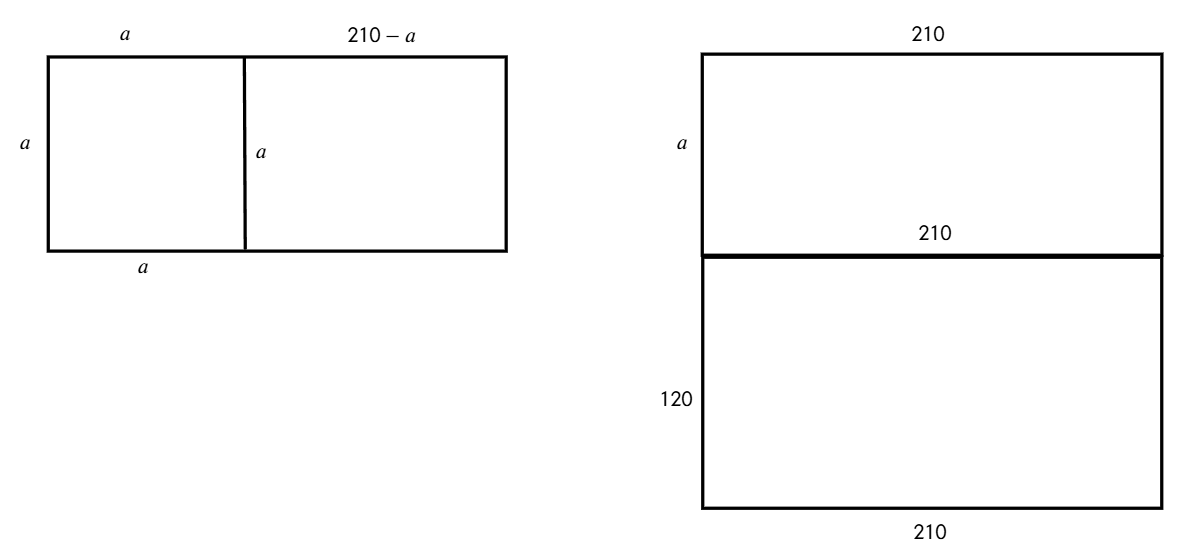
\includegraphics[scale=0.35]{kv4.png}}
\end{figure}\\
Если у прямоугольника периметр равен 420 см, то его стороны в сумме дают $420:2=210$см, то есть они равны $a$ и $210-a.$ Так как после отрезания получился квадрат, всего его стороны равны $a$ (см. левый рисунок). Тогда одна из сторон исходного прямоугольника была равна $a+210-a=210$см. Поэтому у прикладываемого прямоугольника вторая сторона равна $660:2-210=120$см (см. правый рисунок). Так как после прикладывания получился квадрат, должно выполняться равенство $a+120=210,\ a=210-120=90$см. Таким образом, исходный прямоугольник имел размеры $90\text{ см}\times210\text{ см}.$\\
331.\begin{figure}[ht!]
\center{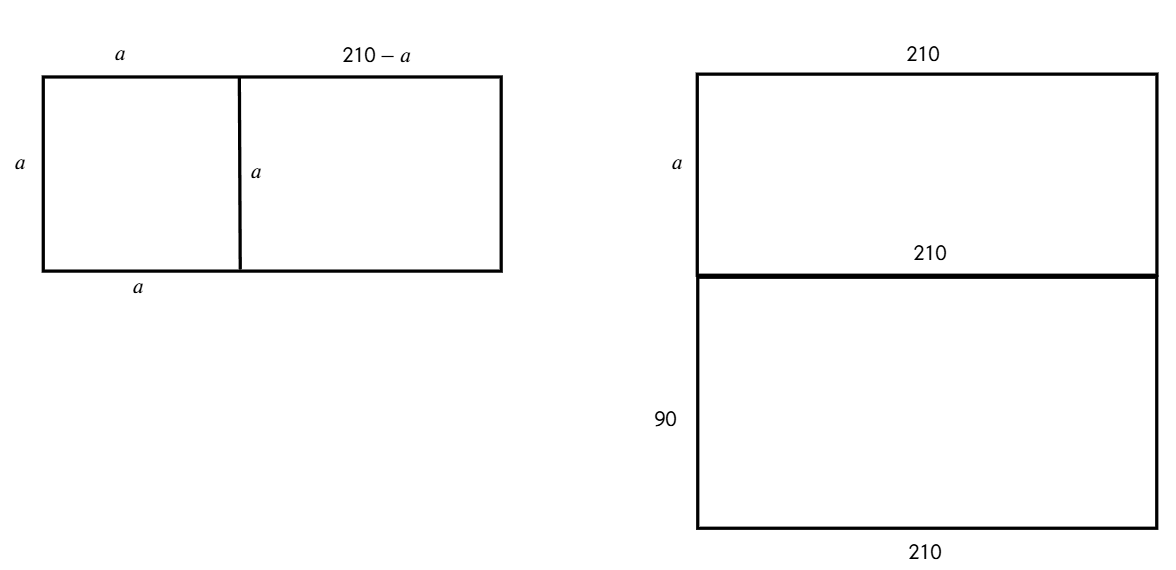
\includegraphics[scale=0.35]{kv5.png}}
\end{figure}\\
Если у прямоугольника периметр равен 420 см, то его стороны в сумме дают $420:2=210$см, то есть они равны $a$ и $210-a.$ Так как после отрезания получился квадрат, всего его стороны равны $a$ (см. левый рисунок). Тогда одна из сторон исходного прямоугольника была равна $a+210-a=210$см. Поэтому у прикладываемого прямоугольника вторая сторона равна $600:2-210=90$см (см. правый рисунок). Так как после прикладывания получился квадрат, должно выполняться равенство $a+90=210,\ a=210-90=120$см. Таким образом, исходный прямоугольник имел размеры $120\text{ см}\times210\text{ см}.$\\
332. Май содержит 4 полных недели и ещё три дня. Раз суббот было больше, чем четвергов, суббота в эти три дня попала, а четверг --- нет. Это могло произойти только если суббота была 29.05 или 30.05. Тогда в первом случае 1.05 было также субботой, а во втором --- пятницей (прошло 28 и 29 дней соответственно). Построим цепочку для невисокосного и високосного года: $1.05\stackrel{-30}{\rightarrow}1.04\stackrel{-31}{\rightarrow}1.03
\stackrel{-28(-29)}{\rightarrow}1.02\stackrel{-2}{\rightarrow}30.01.$
В невисокосном году надо "отмотать назад" $30+31+28+2=91$ день, а в високосном --- $30+31+29+2=92.$ Так как 91 делится на 7, а 92 даёт остаток 1, в первом случае 30.01 могло быть субботой или пятницей, а во втором --- пятницей или четвергом. Значит, все возможные ответы --- это четверг, пятница и суббота.\\
333. Май содержит 4 полных недели и ещё три дня. Раз пятниц было больше, чем сред, пятница в эти три дня попала, а среда --- нет. Это могло произойти только если пятница была 29.05 или 30.05. Тогда в первом случае 1.05 было также пятницей, а во втором --- четвергом (прошло 28 и 29 дней соответственно). Построим цепочку для невисокосного и високосного года: $1.05\stackrel{-30}{\rightarrow}1.04\stackrel{-31}{\rightarrow}1.03
\stackrel{-28(-29)}{\rightarrow}1.02\stackrel{-2}{\rightarrow}30.01.$
В невисокосном году надо "отмотать назад" $30+31+28+2=91$ день, а в високосном --- $30+31+29+2=92.$ Так как 91 делится на 7, а 92 даёт остаток 1, в первом случае 30.01 могло быть пятницей или четвергом, а во втором --- четвергом или средой. Значит, все возможные ответы --- это среда, четверг и пятница.\\
334.\begin{figure}[ht!]
\center{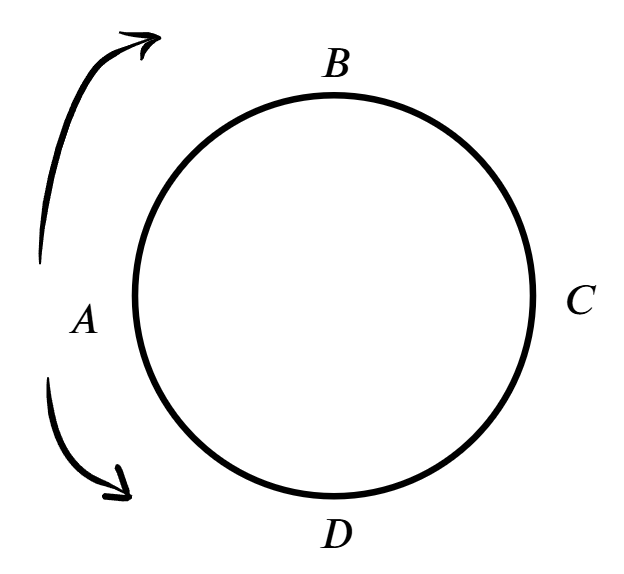
\includegraphics[scale=0.35]{krug3.png}}
\end{figure}\\
Пусть они встречаются в точках $A,\ B,\ C$ и $D.$ Тогда пока первый ездок проезжает дугу $AB,$ второй проезжает дугу $ADCB,$ пока первый проезжает дугу $BC,$ второй проезжает дугу $BADC,$ пока первый проезжает дугу $CD,$ второй проезжает дугу $CBAD$ и пока первый проезжает дугу $DA,$ второй проезжает дугу $DCBA.$ Тогда за то время, пока первый проехал дуги $AB,\ BC,\ CD$ и $DA,$ то есть полный круг, второй проедет дуги $ADCB,\ BADC,\ CBAD,$ и $DCBA,$ то есть три круга. Значит, скорость Максима может быть в три раза больше или в три раза меньше, чем скорость тренера, то есть $12\cdot3=36$км/ч или $12:3=4$км/ч.\\
335.\begin{figure}[ht!]
\center{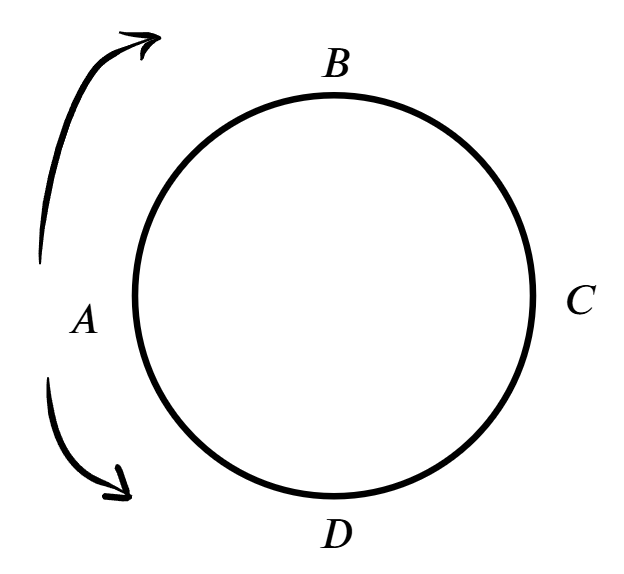
\includegraphics[scale=0.35]{krug3.png}}
\end{figure}\\
Пусть они встречаются в точках $A,\ B,\ C$ и $D.$ Тогда пока первый ездок проезжает дугу $AB,$ второй проезжает дугу $ADCB,$ пока первый проезжает дугу $BC,$ второй проезжает дугу $BADC,$ пока первый проезжает дугу $CD,$ второй проезжает дугу $CBAD$ и пока первый проезжает дугу $DA,$ второй проезжает дугу $DCBA.$ Тогда за то время, пока первый проехал дуги $AB,\ BC,\ CD$ и $DA,$ то есть полный круг, второй проедет дуги $ADCB,\ BADC,\ CBAD,$ и $DCBA,$ то есть три круга. Значит, скорость Максима может быть в три раза больше или в три раза меньше, чем скорость тренера, то есть $15\cdot3=45$км/ч или $15:3=5$км/ч.\\
336. Нам подходят кубики, у которых окрашено 0 или 2 грани (больше быть не может). Первые кубики --- это кубики внутри параллелепипеда, их $2\cdot2\cdot3=12$ штук. Вторые кубики --- это кубики, расположенные вдоль рёбер, кроме первого и последнего (у них покрашено по 3 грани). Таких кубиков $(2+2+3)\cdot4=28.$ Значит, всего подходящих кубиков $12+28=40$ штук.\\
337. Нам подходят кубики, у которых окрашено 0 или 2 грани (больше быть не может). Первые кубики --- это кубики внутри параллелепипеда, их $2\cdot3\cdot3=18$ штук. Вторые кубики --- это кубики, расположенные вдоль рёбер, кроме первого и последнего (у них покрашено по 3 грани). Таких кубиков $(2+3+3)\cdot4=32.$ Значит, всего подходящих кубиков $18+32=50$ штук.\\
338. Рассмотрим следующую цепочку: $19.05.24\stackrel{+365}{\rightarrow}19.05.25\stackrel{-30}{\rightarrow}19.04.25
\stackrel{-31}{\rightarrow}19.03.25.$ Значит, через $365-30-31=304$ дня будет 19 марта, поэтому и через 300 дней тоже будет март.\\
339. Рассмотрим следующую цепочку: $19.05.24\stackrel{+365}{\rightarrow}19.05.25\stackrel{-30}{\rightarrow}19.04.25.$ Значит, через $365-30=335$ дня будет 19 апреля, поэтому и через 330 дней тоже будет апрель.\\
340. В Хабаровске на $17-10=7$ часов больше времени, чем в Брянске, и на $15-10=5$ часов времени больше, чем в Кургане, значит в Кургане на $7-5=2$ часа времени больше, чем в Брянске. Таким образом, путешественник потратил
$03:46-12:01+2:00=17$ часов 45 минут.\\
341. В Хабаровске на $17-10=7$ часов больше времени, чем в Брянске, и на $15-10=5$ часов времени больше, чем в Кургане, значит в Кургане на $7-5=2$ часа времени больше, чем в Брянске. Таким образом, путешественник потратил
$05:45-13:23-2:00=14$ часов 22 минуты.
\newpage
